% =============================================================================
% 流体力学（水力学）自学讲义 · 第 5 部分
% 第五章 5.1--5.2：紊流概论与壁面速度分布
% 模式：passive-study · 主题：teal · 图示：TikZ 重绘
% =============================================================================
\documentclass[aspectratio=169,10pt]{beamer}
\usepackage[teal]{template-lib/template-lib}
\uselayout{text}\uselayout{eq}\uselayout{twocol}\uselayout{1img}\uselayout{table}
\usetikzlibrary{arrows.meta,calc,positioning,patterns,decorations.pathmorphing,decorations.pathreplacing,decorations.markings}

% ── 记号缩写 ─────────────────────────────────────────────────────────────────
\newcommand{\rd}{\,\mathrm{d}}
\newcommand{\dd}[2]{\frac{\mathrm{d}#1}{\mathrm{d}#2}}
\newcommand{\pd}[2]{\frac{\partial #1}{\partial #2}}
\newcommand{\DDt}[1]{\frac{\mathrm{D}#1}{\mathrm{D}t}}
\newcommand{\grad}{\nabla}
\newcommand{\divg}{\nabla\!\cdot}
\newcommand{\vc}[1]{\boldsymbol{#1}}
\newcommand{\Real}{\mathbb{R}}
\newcommand{\Rey}{\mathit{Re}}
\newcommand{\atm}{\mathrm{atm}}
\newcommand{\proofskipnote}{\footnote{\scriptsize 非数学背景读者：本帧为\emph{推导细节}，第一遍可先跳过，记住本帧\emph{要点}即可。}}

% 本地化模板中的 takeaway 标签。
\renewcommand{\TLtakeaway}[1]{%
  \vspace{0.25em}%
  \begin{tikzpicture}
    \node[fill=TLaccentLight, rounded corners=3pt, inner sep=7pt,
          text width=\dimexpr\linewidth-14pt\relax, align=justify] {%
      \small\textcolor{TLaccent}{\textbf{要点。}} #1%
    };
  \end{tikzpicture}%
  \vspace{0.1em}%
}

\TLsetfoot{流体力学（水力学）\textperiodcentered{} 自学讲义 \textperiodcentered{} 第 5 部分：紊流概论·壁面速度分布}

\begin{document}

% =============================================================================
% A. 标题 + 如何使用 + 承前
% =============================================================================
\TLtitlecenter
  {紊流概论与壁面速度分布}
  {流体力学（水力学）自学讲义 \textperiodcentered{} 第 5 部分\\（第五章 5.1--5.2：紊流概论与壁面速度分布）}
  {本轮 PASS A：先建直觉与 5.1 紊流概论}
  {passive-study 自学讲义}

\begin{frame}{如何使用本讲义}
  本讲义研究\TLterm{紊流}：它不是“水流看起来很乱”这么简单，而是要回答乱流怎样产生、怎样取平均、为什么会带来额外切应力。
  \begin{columns}[T]
    \column{0.56\textwidth}
      \begin{itemize}
        \item 非流体背景读者，请先读下一节“先建直觉”。
        \item 带 \proofskipnote 的推导帧可第一遍略读，第二遍逐行核查。
        \item 本轮只写 A--C：开场、直觉、5.1 紊流概论。
        \item 式号用 R1, R2, \dots 标记；R 表示 Reynolds / turbulence。
      \end{itemize}
    \column{0.44\textwidth}
      \centering
      \begin{tikzpicture}[scale=0.52,>={Stealth[length=5pt]}]
        \node[draw=TLprimary,fill=TLprimaryTint,rounded corners=2pt,inner sep=4pt] (why) at (0,1.0) {先看可见现象};
        \node[draw=TLprimary,fill=white,rounded corners=2pt,inner sep=4pt] (avg) at (0,0) {再做时均描述};
        \node[draw=TLaccent,fill=TLaccentLight,rounded corners=2pt,inner sep=4pt] (stress) at (0,-1.0) {最后解释附加应力};
        \draw[->,TLprimaryDark,thick] (why)--(avg);
        \draw[->,TLprimaryDark,thick] (avg)--(stress);
      \end{tikzpicture}
  \end{columns}
  \TLtakeaway{阅读顺序是“层流/紊流直觉 $\to$ 雷诺数判据 $\to$ 时均分解 $\to$ 雷诺应力与混合长”。}
\end{frame}

\begin{frame}{承前（前置知识）}
  本章会把前几部分的粘性、动量和水头语言接到紊流上；后面用到时不要求你回翻。
  \begin{center}
  \vspace{-2pt}
  \footnotesize
  \setlength{\tabcolsep}{4pt}
  \renewcommand{\arraystretch}{0.88}
  \begin{tabular}{@{}p{0.31\textwidth}p{0.63\textwidth}@{}}
    \toprule
    前置对象 & 本章中的用法 \\
    \midrule
    \TLterm{N-S 方程} & 粘性流体的瞬时动量方程；做时均后会多出脉动贡献 \\
    \TLterm{动量定理} & 用“冲量 = 动量变化”解释流层之间的动量交换 \\
    \TLterm{应力张量} & 切应力下标 $\tau_{yx}$ 表示“垂直于 $y$ 的面上、沿 $x$ 的应力” \\
    \TLterm{水头损失} $h_w$ & 真实粘性流动沿程损失机械能；紊流会显著增加损失 \\
    \TLterm{运动粘度} $\nu$ & $\nu=\mu/\rho$，把动力粘度与密度合并，便于写雷诺数 \\
    \TLterm{牛顿内摩擦} & 层流中 $\tau=\mu\,\dd{u}{y}$；紊流时均场不能直接套用 \\
    \TLterm{断面平均流速} $v$ & 圆管雷诺数用 $v$ 与管径 $d$ 作参考量 \\
    \TLterm{过水断面/均匀流} & 用面积 $A$、湿周 $\chi$ 与水力半径 $R$ 描述非圆断面 \\
    \bottomrule
  \end{tabular}
  \end{center}
  \vspace{-2pt}
  \small $\displaystyle \tau=\mu\,\dd{u}{y},\qquad \nu=\frac{\mu}{\rho},\qquad Q=vA.$
  \vspace{-2pt}
  \TLtakeaway{本章不是推翻前几章，而是在“粘性 + 动量 + 断面平均”的语言上增加脉动这一层。}
\end{frame}

% =============================================================================
% B. 先建直觉
% =============================================================================
\TLsection{先建直觉 · 层流与紊流（新手先读）}

\begin{frame}{倒蜂蜜与大河：先分清两种流态}
  \TLterm{层流}像慢慢倒出的蜂蜜：相邻流层大致并排滑动。 \TLterm{紊流}像大河奔涌：流体微团会横向掺混，路径不再规整。
  \begin{center}
  \begin{tikzpicture}[scale=0.74,>={Stealth[length=4pt]}]
    \foreach \x/\title in {-4/层流,0/过渡,4/紊流}{
      \draw[fill=TLprimaryTint,draw=TLprimary,thick,rounded corners=5pt] (\x-1.55,-0.55) rectangle (\x+1.55,0.55);
      \node[TLinkSoft] at (\x,0.92) {\title};
      \draw[TLprimaryDark,thick] (\x-1.55,0.62)--(\x+1.55,0.62);
      \draw[TLprimaryDark,thick] (\x-1.55,-0.62)--(\x+1.55,-0.62);
    }
    \draw[TLaccent,thick] (-5.35,0)--(-2.65,0);
    \draw[TLaccent,thick,decorate,decoration={snake,amplitude=0.35mm,segment length=8mm}]
      (-1.35,0)--(1.35,0.05);
    \draw[TLaccent,thick,decorate,decoration={snake,amplitude=0.8mm,segment length=3.5mm}]
      (2.65,0.25)--(5.35,-0.15);
    \foreach \y in {-0.30,0.0,0.30}{
      \draw[->,TLprimaryDark] (-5.2,\y)--(-4.45,\y);
      \draw[->,TLprimaryDark] (-1.2,\y)--(-0.45,\y+0.05);
      \draw[->,TLprimaryDark] (2.8,\y)--(3.5,\y+0.18);
    }
    \node[align=center,TLinkSoft,text width=11cm] at (0,-1.18)
      {雷诺染色实验：红色染料线越直，流层越不掺混；染料线破碎扩散，说明流体微团在横向交换。};
  \end{tikzpicture}
  \end{center}
  \TLtakeaway{层流/紊流的第一判断不是公式，而是“相邻流层是否强烈掺混”。}
\end{frame}

\begin{frame}{雷诺数：惯性与粘性的口算比值}
  想判断“扰动会不会被粘性抹平”，先看\TLterm{雷诺数}。它把促使流体继续乱跑的惯性，与抑制相对运动的粘性放在同一个无量纲比值里。
  \[
    \Rey=\frac{vd}{\nu}.
  \]
  \begin{columns}[T]
    \column{0.52\textwidth}
      \begin{itemize}
        \item 清水近似取 $\nu=1.0\times10^{-6}\,\mathrm{m^2/s}$。
        \item 小管直径 $d=2.0\,\mathrm{cm}=0.020\,\mathrm m$。
        \item 断面平均流速 $v=0.50\,\mathrm{m/s}$。
      \end{itemize}
      \[
        \Rey=\frac{0.50\times0.020}{1.0\times10^{-6}}=1.0\times10^4.
      \]
    \column{0.48\textwidth}
      \centering
      \begin{tikzpicture}[scale=0.75,>={Stealth[length=5pt]}]
        \draw[TLprimaryDark,thick] (-2.2,0)--(2.2,0);
        \draw[fill=TLprimaryTint,draw=TLprimary,thick] (-1.6,-0.35) rectangle (1.6,0.35);
        \draw[->,TLaccent,thick] (-1.35,0)--(-0.25,0) node[midway,above] {$v$};
        \draw[<->,TLinkSoft,thick] (1.75,-0.35)--(1.75,0.35) node[midway,right] {$d$};
        \node[align=center,TLinkSoft,text width=4.6cm] at (0,-1.1)
          {$10^4$ 已明显大于圆管下临界值 $2000$，工程上按紊流处理。};
      \end{tikzpicture}
  \end{columns}
  \TLtakeaway{$\Rey$ 大表示惯性相对强、扰动更难被粘性耗散；$\Rey$ 小表示粘性相对强、流动更容易保持规整。}
\end{frame}

\begin{frame}{脉动：固定探头看到的速度在抖}
  紊流中，即使平均流量保持不变，固定点测到的瞬时速度也会快速抖动。于是我们把瞬时量拆成“慢变化的时均值 + 快速脉动”。
  \[
    u(t)=\bar u+u'(t),\qquad \overline{u'}=0.
  \]
  \begin{center}
  \begin{tikzpicture}[xscale=1.05,yscale=0.72,>={Stealth[length=4pt]}]
    \draw[->,TLprimaryDark,thick] (0,0)--(8.1,0) node[right] {$t$};
    \draw[->,TLprimaryDark,thick] (0,-1.35)--(0,1.65) node[above] {$u$};
    \draw[TLprimary,thick] (0,0.45)--(8,0.45) node[right] {$\bar u$};
    \draw[TLaccent,thick,smooth,domain=0:8,samples=140]
      plot(\x,{0.45+0.45*sin(150*\x)+0.22*sin(47*\x)});
    \draw[dashed,TLinkSoft] (2.2,0.45)--(2.2,1.13);
    \draw[<->,TLinkSoft] (2.38,0.45)--(2.38,1.13) node[midway,right] {$u'$};
    \node[TLinkSoft,align=center,text width=8.5cm] at (4,-1.1)
      {时均不是说瞬时速度不重要，而是把随机抖动对工程作用的平均效果提取出来。};
  \end{tikzpicture}
  \end{center}
  \TLtakeaway{$u'$ 的时间平均为零，但 $u'^2$ 的平均不为零；脉动强度正是紊流“乱”的量化线索。}
\end{frame}

\begin{frame}{速度剖面：层流抛物线，紊流更钝}
  管壁处速度必须满足无滑移条件 $u=0$。层流主要靠分子粘性传递动量，剖面较尖；紊流有横向掺混，管心附近速度更接近平均值，剖面更“钝”。
  \begin{center}
  \begin{tikzpicture}[scale=0.86,>={Stealth[length=5pt]}]
    \draw[TLprimaryDark,thick] (-5.0,-1.2)--(-5.0,1.2);
    \draw[TLprimaryDark,thick] (-5.0,-1.2)--(-1.3,-1.2);
    \draw[TLprimaryDark,thick] (-5.0,1.2)--(-1.3,1.2);
    \draw[TLaccent,thick,smooth,domain=-1:1,samples=80]
      plot({-5+3.2*(1-\x*\x)}, {1.2*\x});
    \node[TLinkSoft] at (-3.2,-1.65) {层流：抛物线};
    \draw[TLprimaryDark,thick] (1.0,-1.2)--(1.0,1.2);
    \draw[TLprimaryDark,thick] (1.0,-1.2)--(4.7,-1.2);
    \draw[TLprimaryDark,thick] (1.0,1.2)--(4.7,1.2);
    \draw[TLaccent,thick,smooth,domain=-1:1,samples=80]
      plot({1+3.15*(1-abs(\x)^7)}, {1.2*\x});
    \node[TLinkSoft] at (2.9,-1.65) {紊流：更钝};
    \draw[->,TLprimaryDark] (-5.0,0)--(-4.1,0) node[above] {$u$};
    \draw[->,TLprimaryDark] (1.0,0)--(1.9,0) node[above] {$u$};
  \end{tikzpicture}
  \end{center}
  \TLtakeaway{紊流剖面更钝，来自横向动量交换；这正是后面雷诺应力和壁面速度分布要解释的现象。}
\end{frame}

\begin{frame}{阅读路径：本轮先到 5.1}
  本轮 PASS A 只讲到“紊流概论”。壁面速度分布的细节会在后续 PASS 接上。
  \begin{center}
  \begin{tikzpicture}[scale=0.66,>={Stealth[length=5pt]}]
    \node[draw=TLprimary,fill=TLprimaryTint,rounded corners=2pt,minimum width=2.7cm,minimum height=0.72cm] (a) at (-4.4,0.6) {$\star$ 雷诺数};
    \node[draw=TLprimary,fill=TLprimaryTint,rounded corners=2pt,minimum width=2.7cm,minimum height=0.72cm] (b) at (-1.45,0.6) {$\star$ 时均分解};
    \node[draw=TLprimary,fill=TLprimaryTint,rounded corners=2pt,minimum width=2.7cm,minimum height=0.72cm] (c) at (1.5,0.6) {$\star$ 雷诺应力};
    \node[draw=TLaccent,fill=TLaccentLight,rounded corners=2pt,minimum width=2.7cm,minimum height=0.72cm] (d) at (4.45,0.6) {混合长};
    \draw[->,TLprimaryDark,thick] (a)--(b);
    \draw[->,TLprimaryDark,thick] (b)--(c);
    \draw[->,TLprimaryDark,thick] (c)--(d);
    \node[draw=TLprimary,fill=white,rounded corners=2pt,minimum width=2.7cm,minimum height=0.72cm] (e) at (-2.1,-0.85) {后续：$u^+=y^+$};
    \node[draw=TLprimary,fill=white,rounded corners=2pt,minimum width=2.7cm,minimum height=0.72cm] (f) at (1.0,-0.85) {后续：对数律};
    \node[TLinkSoft,align=center,text width=9.8cm] at (0,-1.72)
      {$\star$ 为第一遍必读；带脚注的推导帧可第一遍先抓目标和结论，第二遍逐行复算。假定背景：高等数学、线性代数、大学物理。};
  \end{tikzpicture}
  \end{center}
  \TLtakeaway{先掌握“为何要时均、为何有附加应力”；半经验模型的细节可在第二遍阅读时再补齐。}
\end{frame}

% =============================================================================
% C. 5.1 紊流概论
% =============================================================================
\TLsection{5.1 紊流概论}

\begin{frame}{C1 雷诺实验：用一条红线看见流态}
  \TLterm{雷诺实验}把红色染料注入恒定圆管流。染料线是否保持清晰，直接显示流层是否发生横向掺混。
  \begin{columns}[T]
    \column{0.58\textwidth}
      \centering
      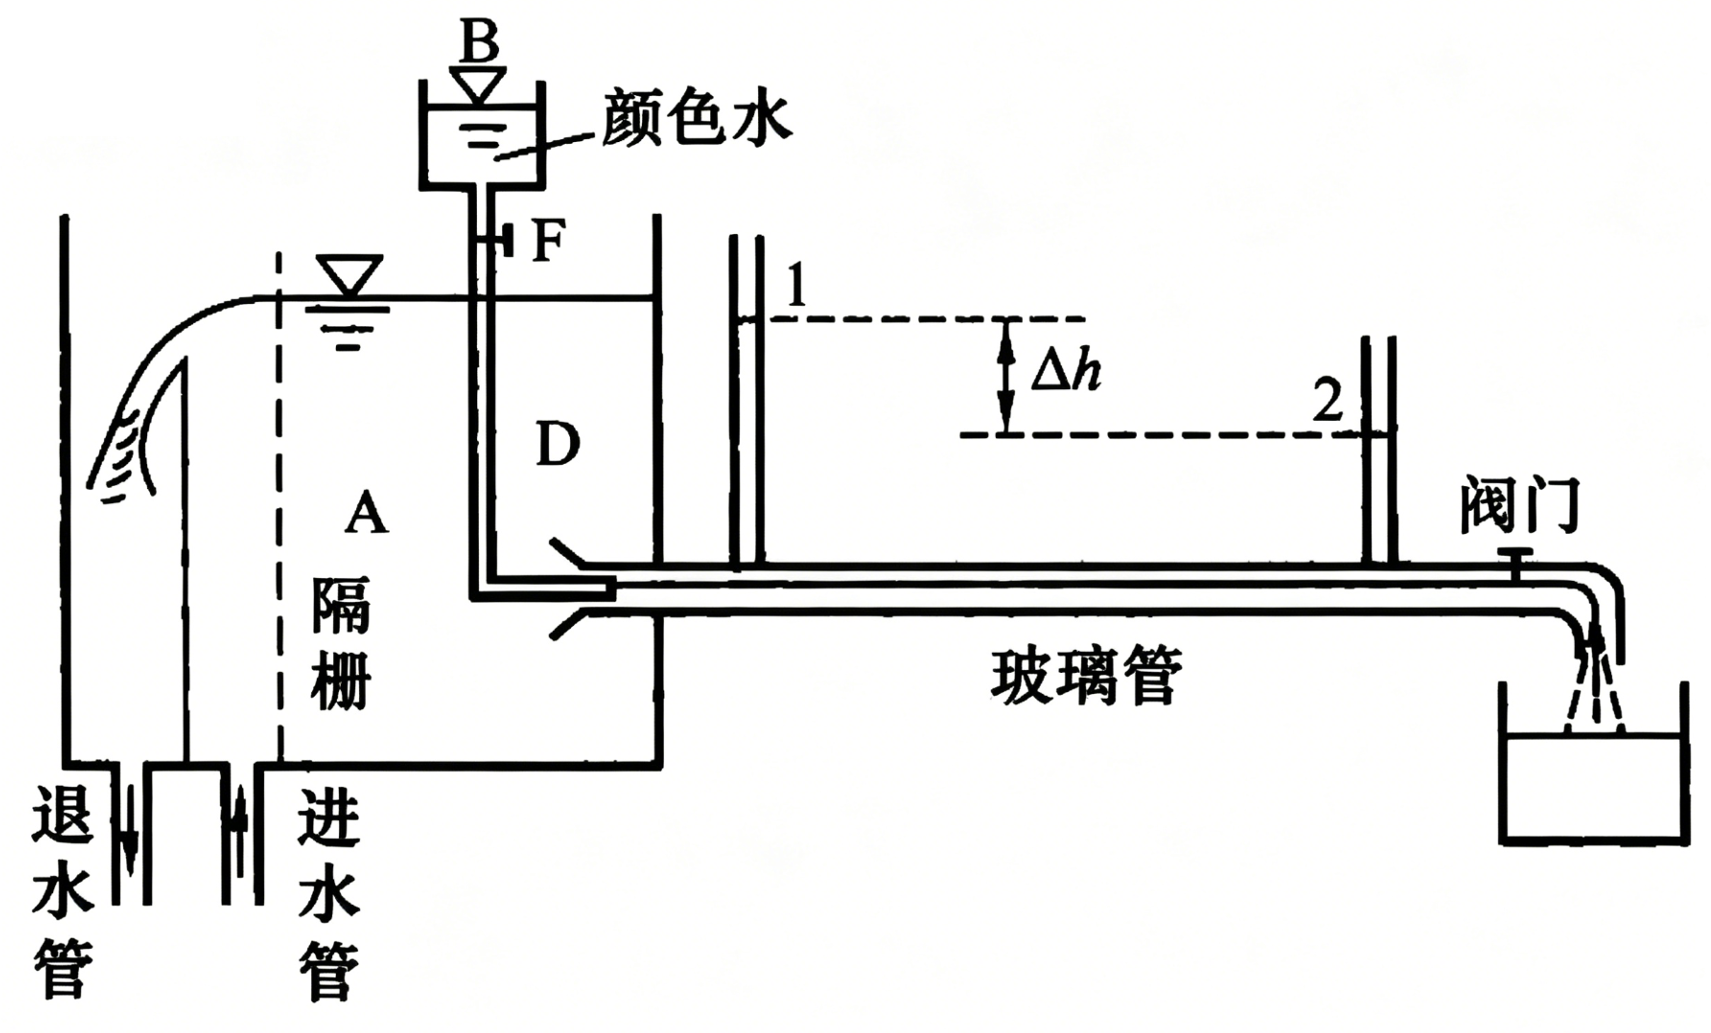
\includegraphics[width=\linewidth,height=0.45\textheight,keepaspectratio]{slides_assets/fluid_deck05/reynolds-apparatus.png}\\
      {\scriptsize 图：源讲义原图}
    \column{0.42\textwidth}
      \footnotesize
      \begin{tabular}{@{}ll@{}}
        \toprule
        流速范围 & 红色染料线 \\
        \midrule
        $v<v_c$ & 直线，几乎不扩散 \\
        $v\gtrsim v_c$ & 弯曲，仍可辨认 \\
        $v$ 很大 & 破碎，迅速染红全管 \\
        \bottomrule
      \end{tabular}
      \vspace{6pt}

      \begin{tikzpicture}[scale=0.58,>={Stealth[length=4pt]}]
        \foreach \y/\lab in {0.9/层流,0/过渡,-0.9/紊流}{
          \draw[TLprimary,thick] (-1.7,\y+0.26)--(1.7,\y+0.26);
          \draw[TLprimary,thick] (-1.7,\y-0.26)--(1.7,\y-0.26);
          \node[TLinkSoft,left] at (-1.9,\y) {\lab};
        }
        \draw[TLaccent,thick] (-1.55,0.9)--(1.55,0.9);
        \draw[TLaccent,thick,decorate,decoration={snake,amplitude=0.35mm,segment length=7mm}]
          (-1.55,0)--(1.55,0.04);
        \draw[TLaccent,thick,decorate,decoration={snake,amplitude=0.8mm,segment length=3mm}]
          (-1.55,-0.78)--(1.55,-1.02);
      \end{tikzpicture}
  \end{columns}
  \TLtakeaway{雷诺实验的核心观察是：流速足够大时，红线不再代表单一流层，而是被横向脉动撕碎并掺混。}
\end{frame}

\begin{frame}{C2 雷诺数：定义、量纲与临界值}
  目标：把“流速、管径、密度、粘度都会影响流态”压缩成一个无量纲指标，并说明工程判据的来源。\proofskipnote
  \begin{columns}[T]
    \column{0.54\textwidth}
      \[
        \Rey=\frac{\rho v d}{\mu}=\frac{vd}{\nu}
        \tag{R1}
      \]
      这里 $d$ 是圆管直径，$v$ 是断面平均流速，$\nu=\mu/\rho$。
      \[
        \left[\frac{\rho vd}{\mu}\right]
        =\frac{(\mathrm{kg/m^3})(\mathrm{m/s})(\mathrm m)}
        {\mathrm{kg/(m\,s)}}=1.
        \tag{R2}
      \]
    \column{0.46\textwidth}
      \footnotesize
      \begin{tabular}{@{}ll@{}}
        \toprule
        量 & 含义 \\
        \midrule
        $v_{cr}'$ & 层流增速后进入过渡的上临界流速 \\
        $v_c$ & 紊流降速后回到层流的下临界流速 \\
        $\Rey_c$ & 圆管下临界雷诺数，约 $2000$ \\
        \bottomrule
      \end{tabular}
      \[
        \Rey_c=\frac{v_c d}{\nu}\approx2000.
        \tag{R3}
      \]
      工程中常用 $\Rey<2000$ 判为层流；$\Rey$ 更大时，工程上通常按紊流处理。
  \end{columns}
  \TLtakeaway{$\Rey$ 不是绝对开关；它是流动失稳倾向的指标。下临界值稳定，所以下临界常被用作保守判据。}
\end{frame}

\begin{frame}{C3 非圆断面：水力半径给参考长度}
  圆管用直径 $d$ 很自然；明渠或非圆管没有唯一“直径”。水力学用\TLterm{水力半径}把面积和壁面接触长度合成参考长度。
  \begin{columns}[T]
    \column{0.50\textwidth}
      \[
        R=\frac{A}{\chi}
        \tag{R4}
      \]
      这里 $A$ 是过水断面面积，$\chi$ 是\TLterm{湿周}，即水流与固体边界接触的长度。
      \[
        R_{\text{圆管}}
        =\frac{\pi d^2/4}{\pi d}
        =\frac d4.
        \tag{R5}
      \]
      广义写法是
      \[
        \Rey=\frac{\rho U L}{\mu}.
        \tag{R6}
      \]
    \column{0.50\textwidth}
      \centering
      \begin{tikzpicture}[scale=0.76,>={Stealth[length=5pt]}]
        \draw[fill=TLprimaryTint,draw=TLprimary,thick] (-1.3,0) circle (0.9);
        \draw[TLaccent,thick] (-0.4,0)--(0.5,0) node[midway,above] {$d/2$};
        \node[TLinkSoft] at (0,-1.28) {满圆管：$\chi=\pi d$};
        \draw[fill=TLprimaryTint,draw=TLprimary,thick] (1.6,-0.45) rectangle (4.2,0.75);
        \draw[TLprimaryDark,thick] (1.6,0.75)--(4.2,0.75);
        \draw[TLaccent,thick] (1.6,-0.45)--(1.6,0.75)--(4.2,0.75)--(4.2,-0.45);
        \node[TLinkSoft,align=center,text width=4.3cm] at (2.9,-1.28)
          {明渠：湿周只数固体接触边界};
      \end{tikzpicture}
      \vspace{2pt}

      以 $R$ 为参考长度时，圆管下临界值从 $2000$ 变为约 $500$。非圆管和明渠工程判据常近似取 $\Rey_R\approx500$。
  \end{columns}
  \TLtakeaway{讨论临界雷诺数前，必须先说清参考速度 $U$ 和参考长度 $L$；换了 $L$，数值门槛也会换。}
\end{frame}

\begin{frame}{C4 物理意义：扰动、压差与涡体}
  $\Rey$ 的大白话意义是\TLterm{惯性力/粘性力之比}。惯性让扰动继续发展，粘性把相对运动耗散掉；两者竞争决定扰动能否长大。
  \begin{columns}[T]
    \column{0.50\textwidth}
      \begin{itemize}
        \item 密度大、速度大、尺度大：扰动携带的动量更难被抹平。
        \item 动力粘度大：相同速度梯度下切应力更大，更容易稳定流动。
        \item 流线一旦弯曲，凸侧通道变细，速度升高、压强降低；凹侧相反。
        \item 压差继续放大弯曲，涡体若不被粘性耗散，就可能发展成紊流。
      \end{itemize}
    \column{0.50\textwidth}
      \centering
      \begin{tikzpicture}[scale=0.74,>={Stealth[length=5pt]}]
        \foreach \y in {-0.75,-0.35,0.05,0.45,0.85}{
          \draw[TLprimaryDark,thick] (-2.2,\y) .. controls (-0.8,\y+0.22) and (0.2,\y-0.22) .. (1.5,\y+0.1);
        }
        \draw[TLaccent,thick,->] (-0.55,0.05) .. controls (-0.1,0.65) and (0.65,0.58) .. (0.78,0.02);
        \draw[TLaccent,thick,->] (0.78,0.02) .. controls (0.7,-0.55) and (-0.15,-0.50) .. (-0.55,0.05);
        \node[TLaccent] at (0.15,0.05) {涡体};
        \node[TLinkSoft,align=center,text width=3.0cm] at (-1.25,1.35) {凸侧：流管窄\\速度大、压强小};
        \node[TLinkSoft,align=center,text width=3.0cm] at (1.55,-1.15) {凹侧：流管宽\\速度小、压强大};
        \draw[->,TLinkSoft,thick] (-0.9,1.0)--(-0.25,0.55);
        \draw[->,TLinkSoft,thick] (1.2,-0.8)--(0.55,-0.35);
      \end{tikzpicture}
  \end{columns}
  \TLtakeaway{紊流形成不是“速度大所以乱”一句话；关键是扰动产生后，惯性能否压过粘性的耗散能力。}
\end{frame}

\begin{frame}{C5a 时均化：把瞬时速度拆成两部分}
  目标：把剧烈抖动的瞬时速度拆成时均值与脉动值，并核查脉动平均值为什么为零。\proofskipnote
  \begin{columns}[T]
    \column{0.56\textwidth}
      \[
        \bar u_x=\frac{1}{T}\int_t^{t+T}u_x\,\rd t
        \tag{R7}
      \]
      \[
        u_x'=u_x-\bar u_x,\qquad
        \overline{u_x'}=\overline{u_x-\bar u_x}=0.
        \tag{R8}
      \]
    \column{0.44\textwidth}
      \begin{itemize}
        \item $T$ 要长到覆盖许多脉动周期。
        \item $T$ 也不能长到抹掉时均值本身的缓慢变化。
        \item $\bar u_x$ 描述可稳定测到的平均作用。
        \item $u_x'$ 描述围绕平均值的快速抖动。
      \end{itemize}
      \centering
      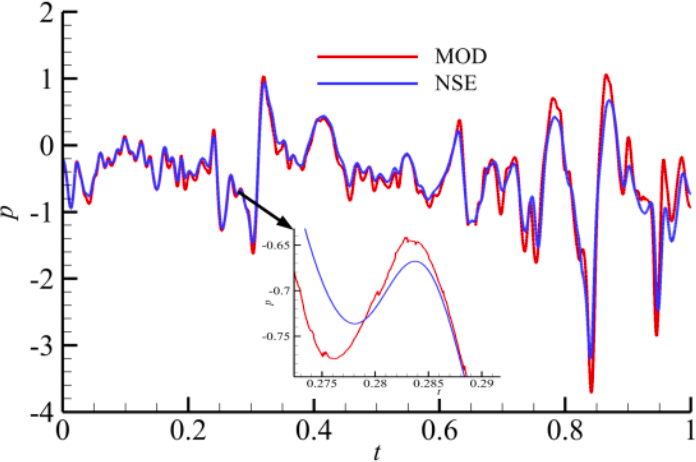
\includegraphics[width=\linewidth,height=0.20\textheight,keepaspectratio]{slides_assets/fluid_deck05/fluctuation.png}\\
      {\scriptsize 图：源讲义原图}
  \end{columns}
  \TLtakeaway{时均分解不是丢弃脉动，而是把“平均作用”和“随机交换”分开记账。}
\end{frame}

\begin{frame}{C5b 时均场：恒定、均匀与牛顿内摩擦的边界}
  完成分解后，紊流描述默认讨论时均场；瞬时场仍在抖动，所以“恒定”和“均匀”都要加上时均限定。
  \begin{columns}[T]
    \column{0.52\textwidth}
      \[
        I_x=\sqrt{\overline{u_x'^2}}
        \quad\text{表示 $x$ 向脉动强度。}
        \tag{R9}
      \]
      \begin{itemize}
        \item “恒定紊流”：$\bar u_x,\bar u_y,\bar u_z,\bar p$ 不随时间变。
        \item “均匀紊流”：时均场在空间上满足均匀流假设。
      \end{itemize}
    \column{0.48\textwidth}
      \TLwarnblock{不能直接套牛顿内摩擦}{把 $\tau=\mu\,\dd{u}{y}$ 中的 $u$ 换成 $\bar u$，不能得到紊流时均切应力。}
      \vspace{4pt}

      原因是紊流有横向动量交换，时均切应力除了分子粘性外，还包含后面要推导的雷诺应力。
  \end{columns}
  \TLtakeaway{脉动的平均值为零，不表示脉动没有作用；脉动相关量的平均值正是雷诺应力的来源。}
\end{frame}

\begin{frame}{C6 雷诺应力 Part 1：动量交换图像}
  先建立图像：若时均速度随 $y$ 增大而增大，横向脉动会把低速流体带到高速层，也会把高速流体带到低速层。
  \[
    \dd{\bar u_x}{y}>0.
    \tag{R10}
  \]
  \begin{columns}[T]
    \column{0.50\textwidth}
      \begin{itemize}
        \item 向上脉动：$u_y'>0$，来自下方的流体携带较小 $x$ 向速度，所以 $u_x'<0$。
        \item 向下脉动：$u_y'<0$，来自上方的流体携带较大 $x$ 向速度，所以 $u_x'>0$。
        \item 两种事件都使 $u_x'u_y'<0$，但都在传递 $x$ 向动量。
      \end{itemize}
    \column{0.50\textwidth}
      \centering
      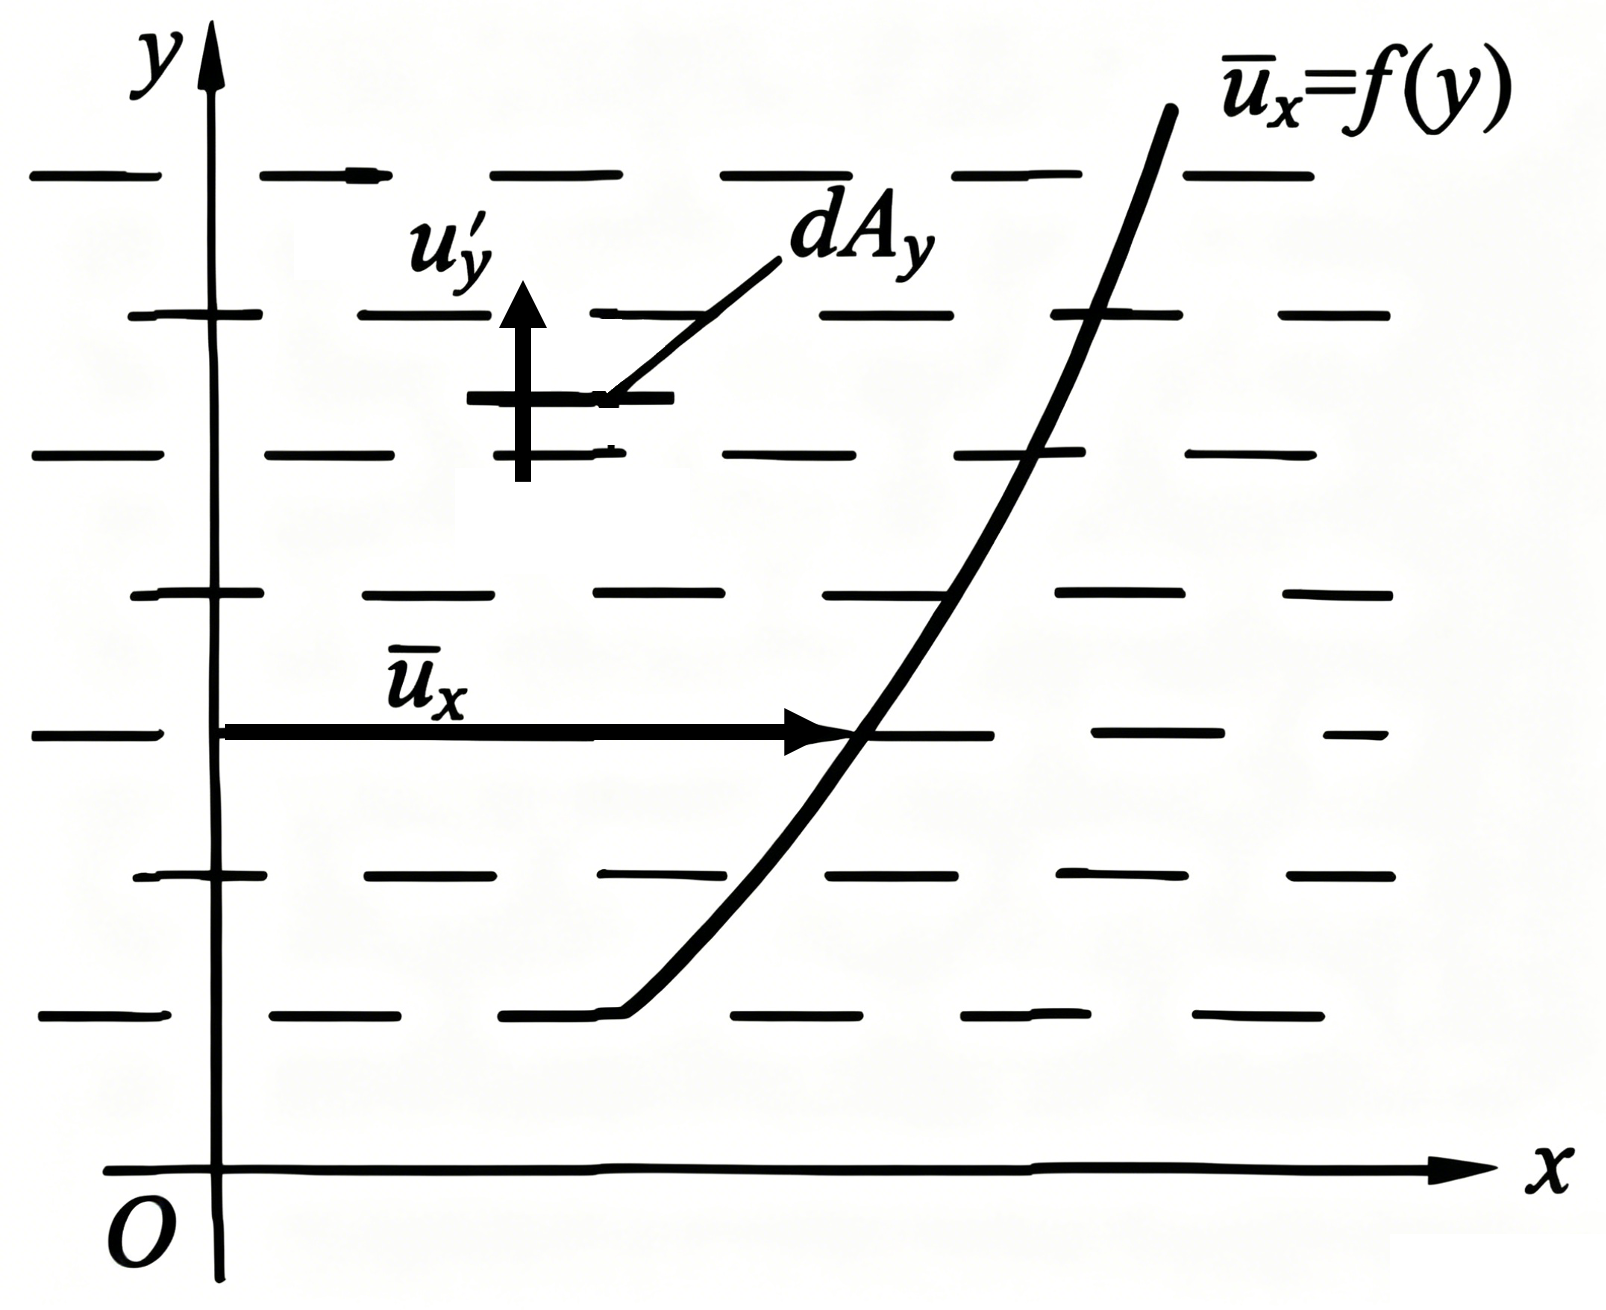
\includegraphics[width=\linewidth,height=0.35\textheight,keepaspectratio]{slides_assets/fluid_deck05/reynolds-stress.png}\\
      {\scriptsize 图：源讲义原图}
  \end{columns}
  \TLtakeaway{雷诺应力不是新的分子力；它是紊流脉动造成的时均动量通量，被写成“应力”的形式。}
\end{frame}

\begin{frame}{C7a 雷诺应力 Part 2：从动量通量到切应力}
  上一帧只说明 $u_x'$ 与 $u_y'$ 近壁常异号。本帧逐步把穿过 $y$ 法向面积的 $x$ 向动量通量写成应力。\proofskipnote
  \begin{enumerate}
    \item 取一个垂直于 $y$ 方向的面积微元 $\rd A_y$。在时间 $\rd t$ 内，由脉动穿过它的有符号质量为
      \[
        \rd m=\rho u_y'\,\rd A_y\,\rd t.
      \]
    \item 这部分质量相对本地时均值多带的 $x$ 向速度是 $u_x'$，所以多带的 $x$ 向动量为
      \[
        \rd P_x'=u_x'\rd m
        =\rho u_x'u_y'\,\rd A_y\,\rd t.
      \]
    \item 除以面积和时间，得到沿 $+y$ 方向输运的 $x$ 向脉动动量通量：
      \[
        j_{xy}^{\mathrm{turb}}
        =\frac{\rd P_x'}{\rd A_y\,\rd t}
        =\rho u_x'u_y'.
        \tag{R11}
      \]
  \end{enumerate}
  \TLtakeaway{到这里还只是“通量”；要变成作用在时均流场上的切应力，还要加上动量守恒中的负号。}
\end{frame}

\begin{frame}{C7b 雷诺应力 Part 2：负号与张量}
  控制体的 $x$ 向动量若被脉动向外带走，控制体内的时均动量就减少。把这个通量改写成“外界对控制体的应力”时，需要取相反号。\proofskipnote
  \[
    \tau_{yx}^{\mathrm{Re}}
    =-\overline{j_{xy}^{\mathrm{turb}}}
    =-\rho\,\overline{u_x'u_y'}.
    \tag{R12}
  \]
  在近壁剪切流中，$u_x'$ 与 $u_y'$ 常反号，所以 $\overline{u_x'u_y'}<0$，从而 $\tau_{yx}^{\mathrm{Re}}>0$。
  {\small
  \[
    \boldsymbol{\tau}^{\mathrm{Re}}
    =-\rho
    \begin{pmatrix}
      \overline{u_x'u_x'} & \overline{u_x'u_y'} & \overline{u_x'u_z'}\\
      \overline{u_y'u_x'} & \overline{u_y'u_y'} & \overline{u_y'u_z'}\\
      \overline{u_z'u_x'} & \overline{u_z'u_y'} & \overline{u_z'u_z'}
    \end{pmatrix}.
    \tag{R13}
  \]
  }
  该张量对称，9 个分量中只有 6 个独立量；对角线是雷诺正应力，非对角线是雷诺切应力。
  \TLtakeaway{负号来自“应力 = 对控制体的作用”与“向外动量通量”的方向约定；不是随意补上的符号。}
\end{frame}

\begin{frame}{C8 雷诺时均方程：多出来的 9 项从哪里来}
  把 N-S 方程中的速度写成 $\bar u_i+u_i'$ 后，线性项可直接平均；非线性的动量输运项会留下脉动乘积。
  \[
    \overline{u_i u_j}
    =\bar u_i\bar u_j+\overline{u_i'u_j'}.
    \tag{R14}
  \]
  第二项无法由时均速度直接给出，所以它成为新未知量。对不可压缩流，时均动量方程可写成
  \[
    \begin{aligned}
    \rho\!\left(\pd{\bar u_i}{t}+\bar u_j\pd{\bar u_i}{x_j}\right)
    &=-\pd{\bar p}{x_i}+\mu\nabla^2\bar u_i+\rho f_i\\
    &\quad+\pd{}{x_j}\!\left(-\rho\overline{u_i'u_j'}\right),
    \qquad i,j\in\{x,y,z\}.
    \end{aligned}
    \tag{R15}
  \]
  对重复的 $j$ 求和；$i,j$ 的 3×3 组合就是形式上多出的 9 项。
  \TLtakeaway{雷诺时均方程形式上比 N-S 多 9 项；这些项不是新假设，而是脉动动量通量取时均后留下的雷诺应力。}
\end{frame}

\begin{frame}{C9 普朗特混合长理论 Part 1：类比分子自由程}
  \TLterm{混合长} $l$ 的作用，是用一个可拟合的长度来描述流体微团在交换动量前能横向“跑多远”。
  \begin{columns}[T]
    \column{0.54\textwidth}
      \begin{itemize}
        \item 分子自由程：分子碰撞前走一小段距离。
        \item 紊流微团：横向脉动后，带着原流层的动量到新位置再混合。
        \item 若 $l$ 很小，时均速度在这段距离内可近似线性变化。
      \end{itemize}
      \[
        \Delta \bar u_x\approx l\,\dd{\bar u_x}{y},
        \qquad
        |u_x'|\sim l\left|\dd{\bar u_x}{y}\right|.
        \tag{R16}
      \]
    \column{0.46\textwidth}
      \centering
      \begin{tikzpicture}[scale=0.74,>={Stealth[length=5pt]}]
        \draw[TLprimaryDark,thick] (-1.9,-1.0)--(1.9,-1.0);
        \draw[TLprimaryDark,thick] (-1.9,1.0)--(1.9,1.0);
        \foreach \y/\len in {-1.0/0.9,0/1.45,1.0/2.0}{
          \draw[->,TLprimary,thick] (-1.7,\y)--++(\len,0);
        }
        \draw[<->,TLaccent,thick] (0.25,-0.75)--(0.25,0.75) node[midway,right] {$l$};
        \fill[TLaccent] (0.25,-0.75) circle (2pt);
        \fill[TLaccent] (0.25,0.75) circle (2pt);
        \node[TLinkSoft,align=center,text width=4.6cm] at (0,-1.55)
          {微团跨过距离 $l$，看到的时均速度差约为斜率乘距离};
      \end{tikzpicture}
  \end{columns}
  \TLtakeaway{混合长理论的第一步是模型假设：用局部速度梯度估算脉动速度量级。}
\end{frame}

\begin{frame}{C10a 混合长理论 Part 2：得到雷诺切应力公式}
  现在把混合长估算代入雷诺应力。这里的 $u$ 表示时均速度，水力学写法常省略横线。\proofskipnote
  \textbf{半经验公式（拟合对象：雷诺切应力）。} 假设简单剪切流、$u_x'$ 与 $u_y'$ 量级相同，且二者在近壁剪切中反相关：
  \[
    |u_x'|=c_1l'\left|\dd{u}{y}\right|,
    \qquad
    |u_y'|=c_2l'\left|\dd{u}{y}\right|.
  \]
  因为 $u_x'u_y'$ 平均为负，
  \[
    -\overline{u_x'u_y'}
    \approx c_1c_2(l')^2\left(\dd{u}{y}\right)^2.
  \]
  把 $c_1c_2(l')^2$ 合并记为 $l^2$，得到
  \[
    \tau^{\mathrm{Re}}
    =\rho l^2\left(\dd{u}{y}\right)^2.
    \tag{R17}
  \]
  \TLtakeaway{普朗特公式不是从 N-S 严格解出；它用可实验拟合的 $l$ 把未知的脉动相关量封闭起来。}
\end{frame}

\begin{frame}{C10b 混合长理论 Part 2：圆管混合长与涡粘模型}
  \textbf{半经验公式（拟合对象：圆管中混合长分布）。} 对半径为 $r_0$ 的圆管，距壁面 $y$ 处常用
  \[
    l\approx \kappa y\sqrt{1-\frac{y}{r_0}},
    \qquad \kappa\approx0.4.
    \tag{R18}
  \]
  \begin{columns}[T]
    \column{0.52\textwidth}
      \textbf{适用假设。}
      \begin{itemize}
        \item 圆管内的壁面剪切紊流。
        \item $y$ 从壁面向管心量起。
        \item $l$ 由实验整理得到，不是普适常数。
      \end{itemize}
    \column{0.48\textwidth}
      \textbf{半经验公式（拟合对象：总切应力）。}
      \[
        \eta=\rho l^2\left|\dd{u}{y}\right|,
        \qquad
        \tau=(\mu+\eta)\dd{u}{y}.
        \tag{R19}
      \]
      这就是\TLterm{布辛涅斯克涡粘模型}；$\eta$ 是\TLterm{涡粘系数}，随流动状态变。
  \end{columns}
  \TLtakeaway{涡粘模型把紊流动量交换写得像“更大的粘度”，但 $\eta$ 不是流体物性，而是流场状态量。}
\end{frame}

% =============================================================================
% D. 5.2 壁面附近的紊流速度分布
% =============================================================================
\TLsection{5.2 壁面附近的紊流速度分布}

\begin{frame}{D1 三分区：近壁陡、管心钝}
  本节要回答的问题是：紊流剖面无法像层流那样精确解出时，壁面附近还能不能抓住主导机制写出可用公式。
  \begin{center}
  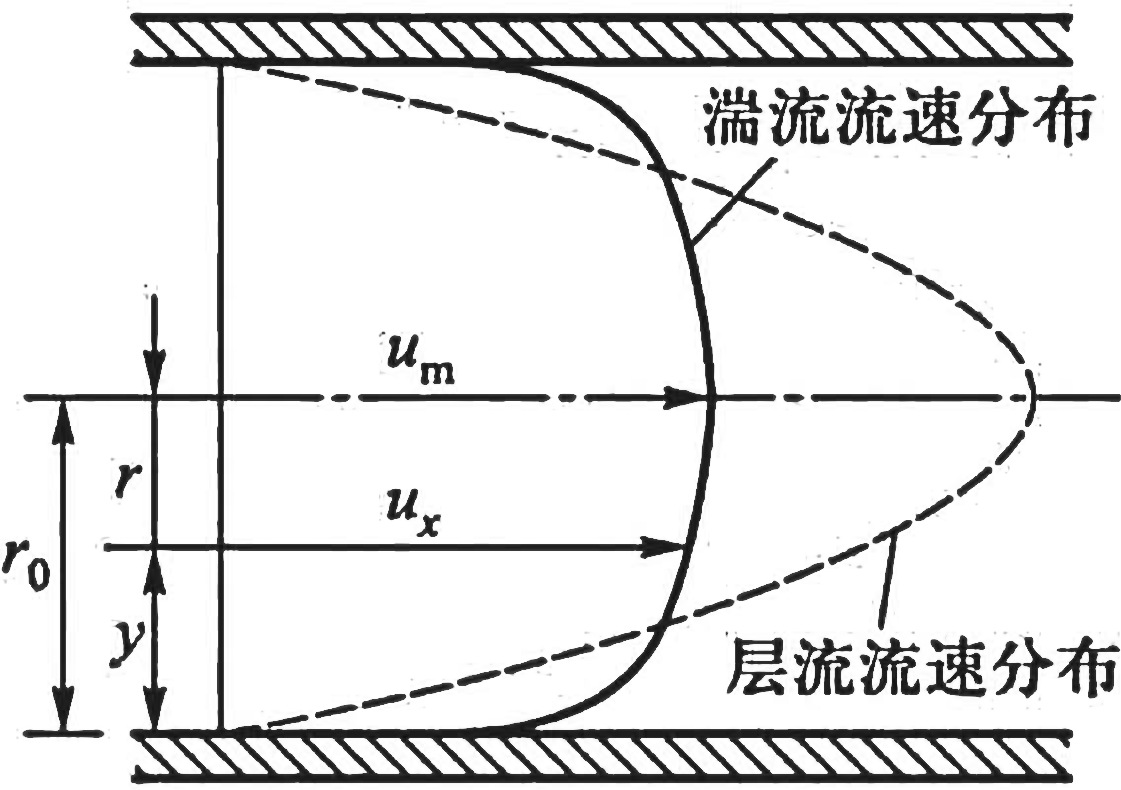
\includegraphics[width=0.72\textwidth,height=0.45\textheight,keepaspectratio]{slides_assets/fluid_deck05/three-zones.png}\\
  {\scriptsize 图：源讲义原图}
  \end{center}
  \TLtakeaway{三分区不是三种流体，而是同一条紊流剖面上主导切应力机制随距壁距离改变。}
\end{frame}

\begin{frame}{D2a 粘性底层：为什么可近似为壁面剪切}
  进度：先只看极靠近壁面的薄层；上一节的总切应力公式中，粘性项占主导，且这一薄层内总切应力近似等于壁面切应力。\proofskipnote
  \begin{columns}[T]
    \column{0.56\textwidth}
      \[
        \tau
        =\mu\dd{u}{y}+\rho l^2\left(\dd{u}{y}\right)^2
        \approx \mu\dd{u}{y}
        \approx \tau_w .
        \tag{R20}
      \]
      这里 $y$ 很小，所以混合长 $l$ 很小，紊流附加切应力相对粘性切应力可忽略；薄层很薄，所以 $\tau$ 沿 $y$ 的变化也可忽略。
    \column{0.44\textwidth}
      \centering
      \begin{tikzpicture}[scale=0.78,>={Stealth[length=5pt]}]
        \fill[TLprimaryTint,draw=TLprimary,thick] (-0.3,0) rectangle (3.1,0.32);
        \node[TLinkSoft] at (1.4,-0.28) {固壁};
        \draw[->,TLprimaryDark,thick] (0,0.32)--(0,2.8) node[above] {$y$};
        \draw[->,TLprimaryDark,thick] (0,0.32)--(3.2,0.32) node[right] {$u$};
        \draw[TLaccent,thick] (0,0.32)--(2.55,2.35);
        \draw[dashed,TLinkSoft] (0,0.72)--(2.85,0.72);
        \draw[dashed,TLinkSoft] (0,1.12)--(2.85,1.12);
        \node[TLinkSoft,font=\scriptsize,align=center] at (2.4,1.05)
          {薄层内\\$\tau\approx\tau_w$};
        \draw[->,TLaccent,thick] (1.1,0.44)--(1.85,0.44) node[right,font=\scriptsize] {$\tau_w$};
      \end{tikzpicture}
  \end{columns}
  \TLtakeaway{近壁近似的两句话是：粘性主导，所以 $\tau\approx\mu\,\mathrm du/\mathrm dy$；薄层内切应力几乎常数，所以 $\tau\approx\tau_w$。}
\end{frame}

\begin{frame}{D2b 粘性底层：积分得到线性速度分布}
  进度：上一帧得到 $\mu\,\mathrm du/\mathrm dy=\tau_w$；本帧只做积分，并使用无滑移边界条件 $u|_{y=0}=0$。\proofskipnote
  \begin{columns}[T]
    \column{0.58\textwidth}
      \[
        \begin{aligned}
        \mu\dd{u}{y}&=\tau_w,\\
        \rd u&=\frac{\tau_w}{\mu}\rd y,\\
        \int_{0}^{u}\rd u
          &=\frac{\tau_w}{\mu}\int_{0}^{y}\rd y,\\
        u&=\frac{\tau_w}{\mu}y .
        \end{aligned}
        \tag{R21}
      \]
      这就是\TLterm{粘性底层线性速度分布}。
    \column{0.42\textwidth}
      \centering
      \begin{tikzpicture}[scale=0.72,>={Stealth[length=5pt]}]
        \fill[TLprimaryTint,draw=TLprimary,thick] (-0.2,0) rectangle (2.8,0.28);
        \draw[->,TLprimaryDark,thick] (0,0.28)--(0,2.75) node[above] {$y$};
        \draw[->,TLprimaryDark,thick] (0,0.28)--(3.0,0.28) node[right] {$u$};
        \draw[TLaccent,thick] (0,0.28)--(2.45,2.30);
        \node[TLaccent,font=\scriptsize,align=center] at (1.65,1.75)
          {$u=(\tau_w/\mu)y$};
        \fill[TLaccent] (0,0.28) circle (2pt);
        \node[TLinkSoft,font=\scriptsize,align=center] at (1.35,-0.35)
          {无滑移边界\\$u(0)=0$};
      \end{tikzpicture}
  \end{columns}
  \TLtakeaway{线性不是经验拟合，而是近壁“粘性主导 + 切应力近似常数 + 无滑移”的直接积分结果。}
\end{frame}

\begin{frame}{D3 摩阻流速 $u_*$：用壁面切应力构造速度标尺}
  线性式 (R21) 的斜率随工况变。为了把不同工况放到同一张无量纲图上，先用 $\tau_w$ 和 $\rho$ 构造一个有速度量纲的标尺。
  \begin{columns}[T]
    \column{0.54\textwidth}
      \[
        \begin{aligned}
        u_*&=\sqrt{\frac{\tau_w}{\rho}},\\
        \left[\frac{\tau_w}{\rho}\right]
        &=
        \frac{\mathrm{N/m^2}}{\mathrm{kg/m^3}}
        =
        \frac{\mathrm{kg/(m\,s^2)}}{\mathrm{kg/m^3}}\\
        &=\mathrm{m^2/s^2}.
        \end{aligned}
        \tag{R22}
      \]
      因此 $u_*$ 的量纲是 $\mathrm{m/s}$。
      \begin{itemize}
        \item $u_*$ 称为\TLterm{摩阻流速}或 friction velocity。
        \item 它表征壁面对流动施加剪切阻碍的强弱。
      \end{itemize}
    \column{0.46\textwidth}
      \centering
      \begin{tikzpicture}[scale=0.72,>={Stealth[length=5pt]}]
        \fill[TLprimaryTint,draw=TLprimary,thick] (-2.1,-0.25) rectangle (2.1,0.15);
        \draw[->,TLaccent,thick] (-1.5,0.3)--(-0.25,0.3) node[midway,above] {$\tau_w$};
        \node[draw=TLprimary,fill=white,rounded corners=2pt,align=center,minimum width=2.5cm] (scale) at (0,1.15)
          {构造速度标尺\\$u_*=\sqrt{\tau_w/\rho}$};
        \draw[->,TLprimaryDark,thick] (-0.25,0.42)--(scale.south);
        \draw[TLprimaryDark,thick] (-1.65,2.2)--(1.65,2.2);
        \foreach \x in {-1.2,-0.4,0.4,1.2}{
          \draw[->,TLprimary,thick] (\x,1.72)--++(0.35,0);
        }
        \node[TLinkSoft,font=\scriptsize,align=center,text width=4.4cm] at (0,-0.92)
          {$u_*$ 不表示管内某点真的以这个速度流动；它是把壁面剪切强度换成速度单位。};
      \end{tikzpicture}
  \end{columns}
  \TLtakeaway{摩阻流速是构造量，不是实际流速；它让“壁面剪切强弱”可以和速度分布放在同一套无量纲单位里。}
\end{frame}

\begin{frame}{D4 壁面律：粘性底层里的 $u^+=y^+$}
  本帧把 (R21) 改写成无量纲形式。这样不同 $\tau_w,\mu,\rho$ 的近壁线性剖面，会压到同一条直线上。\proofskipnote
  \begin{columns}[T]
    \column{0.54\textwidth}
      \[
        u^+=\frac{u}{u_*},
        \qquad
        y^+=\frac{u_*y}{\nu}.
        \tag{R23}
      \]
      由 (R21) 和 $\nu=\mu/\rho$，
      \[
        \begin{aligned}
        u^+
        &=\frac{u}{u_*}
        =\frac{1}{u_*}\frac{\tau_w}{\mu}y\\
        &=\frac{\rho u_*^2}{\mu}\frac{y}{u_*}
        =\frac{u_*y}{\nu}
        =y^+ .
        \end{aligned}
        \tag{R24}
      \]
      这就是\TLterm{壁面律（粘性底层）}。
    \column{0.46\textwidth}
      \centering
      \begin{tikzpicture}[xscale=1.0,yscale=0.55,>={Stealth[length=5pt]}]
        \draw[->,TLprimaryDark,thick] (0,0)--(4.3,0) node[right] {$\lg y^+$};
        \draw[->,TLprimaryDark,thick] (0,0)--(0,4.2) node[above] {$u^+$};
        \fill[TLprimaryTint] (0,0) rectangle (1.35,4.0);
        \node[font=\scriptsize,TLprimaryDark] at (0.72,3.7) {$y^+\le5$};
        \draw[TLaccent,thick] (0.08,0.18)--(1.05,3.1);
        \node[TLaccent,font=\scriptsize] at (1.38,3.05) {$u^+=y^+$};
        \foreach \x/\lab in {0/1,1/10,2/100,3/1000}{
          \draw[TLinkSoft] (\x,0.07)--(\x,-0.07) node[below,font=\scriptsize] {$\lab$};
        }
        \draw[dashed,TLinkSoft] (0.70,0)--(0.70,4.0);
        \node[TLinkSoft,font=\scriptsize,align=center,text width=4.5cm] at (2.55,1.1)
          {CFD 网格若要解析粘性底层，常要求首层网格中心 $y^+\le1$。};
      \end{tikzpicture}
  \end{columns}
  \TLtakeaway{$y^+$ 是壁面网格的共同语言：它把实际距离 $y$ 换成“按摩阻和粘性缩放后的距壁距离”。}
\end{frame}

\begin{frame}{D5a 对数律推导：核心区的三条输入}
  进度：已经得到粘性底层的线性律；现在进入紊流核心区，粘性剪切相对小，主导项变成混合长给出的雷诺剪切。\proofskipnote
  \textbf{半经验公式（圆管核心区混合长；拟合对象：速度梯度与雷诺剪切，适用假设：充分发展圆管紊流）。}
  \[
    \begin{aligned}
    \tau&\approx\rho l^2\left(\dd{u}{y}\right)^2,\\
    \tau&\approx\tau_w\left(1-\frac{y}{r_0}\right),\\
    l&=\kappa y\sqrt{1-\frac{y}{r_0}} .
    \end{aligned}
    \tag{R25}
  \]
  三条输入分别来自：混合长封闭、圆管切应力线性分布、普朗特圆管混合长。后两条都含有同一个圆管几何因子 $1-y/r_0$。
  \TLtakeaway{圆管中的两个因子 $1-y/r_0$ 会在下一步消掉，这正是对数律能出现的关键。}
\end{frame}

\begin{frame}{D5b 对数律推导：圆管几何因子在哪里}
  目的：在代入前先看清 $y$ 的取法。这里 $y$ 从壁面向管心量起，$r_0$ 是管半径，所以核心区内 $0<y<r_0$。
  \begin{center}
  \begin{tikzpicture}[scale=0.78,>={Stealth[length=5pt]}]
    \draw[TLprimaryDark,thick] (-0.4,-1.25)--(-0.4,1.25);
    \draw[TLprimaryDark,thick] (-0.4,-1.25)--(4.0,-1.25);
    \draw[TLprimaryDark,thick] (-0.4,1.25)--(4.0,1.25);
    \draw[dashed,TLinkSoft] (3.35,-1.25)--(3.35,1.25);
    \node[TLinkSoft,font=\scriptsize] at (3.35,1.55) {管心};
    \draw[<->,TLaccent,thick] (-0.4,-1.55)--(1.15,-1.55) node[midway,below] {$y$};
    \draw[<->,TLinkSoft,thick] (-0.4,1.55)--(3.35,1.55) node[midway,above] {$r_0$};
    \draw[TLaccent,thick] (-0.4,-0.95) -- (3.0,-0.05);
    \node[TLaccent,font=\scriptsize,align=center] at (1.75,-0.68)
      {$\tau=\tau_w(1-y/r_0)$};
    \foreach \x/\len in {0.15/0.8,0.95/1.35,1.75/1.8,2.55/2.05}{
      \draw[->,TLprimary,thick] (\x,0.42)--++(\len*0.42,0);
    }
    \node[TLinkSoft,font=\scriptsize,align=center,text width=8.5cm] at (1.75,-2.15)
      {$y$ 越接近管心，$1-y/r_0$ 越小；同一因子同时影响切应力与混合长。};
  \end{tikzpicture}
  \end{center}
  \TLtakeaway{后面约去 $1-y/r_0$ 时用到的前提，是核心区位置仍满足 $0<y<r_0$。}
\end{frame}

\begin{frame}{D5c 对数律推导：把圆管混合长代入}
  进度：上一帧列出核心区的三条输入；本帧只把 $\tau$ 与 $l$ 代入 $\tau\approx\rho l^2(\mathrm du/\mathrm dy)^2$。\proofskipnote
  \[
    \begin{aligned}
    \rho\!\left[\kappa y\sqrt{1-\frac{y}{r_0}}\right]^2
    \left(\dd{u}{y}\right)^2
    &=
    \tau_w\left(1-\frac{y}{r_0}\right).
    \end{aligned}
    \tag{R26}
  \]
  \begin{center}
  \begin{tikzpicture}[scale=0.72,>={Stealth[length=5pt]}]
    \node[draw=TLprimary,fill=TLprimaryTint,rounded corners=2pt,minimum width=3.0cm,align=center] (mix) at (-3.2,0)
      {混合长模型\\$\rho l^2(\mathrm du/\mathrm dy)^2$};
    \node[draw=TLprimary,fill=white,rounded corners=2pt,minimum width=2.5cm,align=center] (pipe) at (0,0.75)
      {圆管剪切\\$\tau_w(1-y/r_0)$};
    \node[draw=TLprimary,fill=white,rounded corners=2pt,minimum width=2.5cm,align=center] (len) at (0,-0.75)
      {混合长\\$\kappa y\sqrt{1-y/r_0}$};
    \node[draw=TLaccent,fill=TLaccentLight,rounded corners=2pt,minimum width=2.8cm,align=center] (eq) at (3.35,0)
      {同一方程\\两边可约因子};
    \draw[->,TLprimaryDark,thick] (mix)--(eq);
    \draw[->,TLprimaryDark,thick] (pipe)--(eq);
    \draw[->,TLprimaryDark,thick] (len)--(eq);
  \end{tikzpicture}
  \end{center}
  \TLtakeaway{代入后还没有“证明完成”；必须显式展开平方并说明可约去的因子为正。}
\end{frame}

\begin{frame}{D5d 对数律推导：消去圆管因子}
  进度：上一帧得到代入式；本帧展开平方，并利用 $0<y<r_0$ 说明 $1-y/r_0$ 可以约去。\proofskipnote
  \[
    \begin{aligned}
    \rho\kappa^2y^2\left(1-\frac{y}{r_0}\right)
    \left(\dd{u}{y}\right)^2
    &=
    \tau_w\left(1-\frac{y}{r_0}\right),\\
    \rho\kappa^2y^2\left(\dd{u}{y}\right)^2&=\tau_w .
    \end{aligned}
    \tag{R27}
  \]
  因为核心区位置仍满足 $0<y<r_0$，所以 $1-y/r_0>0$。两边同除以这个正因子，不改变等式方向。
  \TLtakeaway{对数律的“奇妙简化”不是跳步：同一个圆管几何因子同时出现在切应力和混合长里，因此可被约去。}
\end{frame}

\begin{frame}{D5e 对数律推导：取正根并积分}
  进度：上一帧已化为 $\rho\kappa^2y^2(\mathrm du/\mathrm dy)^2=\tau_w$；本帧取正根并积分。\proofskipnote
  \[
    \begin{aligned}
    \dd{u}{y}
    &=\frac{1}{\kappa y}\sqrt{\frac{\tau_w}{\rho}}
    =\frac{u_*}{\kappa y},\\
    \int \rd u&=\frac{u_*}{\kappa}\int\frac{\rd y}{y},\\
    u&=\frac{u_*}{\kappa}\ln y+C_1 .
    \end{aligned}
    \tag{R28}
  \]
  速度从壁面向管心增大，所以 $\mathrm du/\mathrm dy>0$，应取正根。
  \TLtakeaway{\textbf{对数律（推导）。} 对数来自 $\int \rd y/y=\ln y$；它不是凭空拟合出来的，但积分常数仍需实验确定。}
\end{frame}

\begin{frame}{D6a 对数律无量纲化：把常数吸收到 $C$}
  目的：把 (R28) 改写为壁面单位，使不同光滑圆管实验能用同一条核心区经验曲线表示。\proofskipnote
  \begin{columns}[T]
    \column{0.58\textwidth}
      因为 $y=y^+\nu/u_*$，
      \[
        \begin{aligned}
        u^+&=\frac{u}{u_*}\\
        &=\frac{1}{\kappa}\ln\!\left(y^+\frac{\nu}{u_*}\right)
          +\frac{C_1}{u_*}\\
        &=\frac{1}{\kappa}\ln y^+ + C .
        \end{aligned}
        \tag{R29}
      \]
      这里的 $C$ 吸收了 $(1/\kappa)\ln(\nu/u_*)+C_1/u_*$，所以无量纲后只剩一个待实验确定的常数。
    \column{0.42\textwidth}
      \centering
      \begin{tikzpicture}[scale=0.76,>={Stealth[length=5pt]}]
        \node[draw=TLprimary,fill=TLprimaryTint,rounded corners=2pt,align=center] (dim) at (-1.6,0)
          {有量纲\\$u=(u_*/\kappa)\ln y+C_1$};
        \node[draw=TLaccent,fill=TLaccentLight,rounded corners=2pt,align=center] (wall) at (2.0,0)
          {壁面单位\\$u^+=(1/\kappa)\ln y^+ + C$};
        \draw[->,TLprimaryDark,thick] (dim)--node[above,font=\scriptsize] {$u_*,\nu$ 缩放} (wall);
      \end{tikzpicture}
  \end{columns}
  \TLtakeaway{无量纲化的目的不是改变物理，而是把工况相关的量并入 $y^+$ 和常数 $C$。}
\end{frame}

\begin{frame}{D6b 光滑管对数律：常数与对数底数}
  目的：给出光滑管核心区最常用的实验常数，并把自然对数到常用对数的换算写清楚。
  \begin{columns}[T]
    \column{0.58\textwidth}
      \textbf{半经验公式（光滑管对数律）（拟合光滑管实验数据，适用 $y^+>70$）。}
      \[
        \begin{aligned}
        u^+&=2.5\ln y^+ +5.5\\
        &=2.5(2.303\,\lg y^+)+5.5\\
        &\approx 5.75\,\lg y^+ +5.5 .
        \end{aligned}
        \tag{R30}
      \]
    \column{0.42\textwidth}
      \centering
      \begin{tikzpicture}[xscale=1.05,yscale=0.58,>={Stealth[length=5pt]}]
        \draw[->,TLprimaryDark,thick] (0,0)--(4.1,0) node[right] {$\lg y^+$};
        \draw[->,TLprimaryDark,thick] (0,0)--(0,4.1) node[above] {$u^+$};
        \fill[TLprimary!10] (2.0,0) rectangle (3.8,3.9);
        \node[font=\scriptsize,TLinkSoft] at (2.9,3.65) {$y^+>70$};
        \draw[TLaccent,thick] (1.85,1.25)--(3.75,3.15);
        \node[TLaccent,font=\scriptsize,align=center] at (2.95,1.55)
          {$u^+=5.75\lg y^+ +5.5$};
        \draw[dashed,TLinkSoft] (1.85,0)--(1.85,3.6);
        \node[TLinkSoft,font=\scriptsize] at (1.85,-0.25) {$70$};
        \foreach \x/\lab in {0/1,1/10,2/100,3/1000}{
          \draw[TLinkSoft] (\x,0.07)--(\x,-0.07) node[below,font=\scriptsize] {$\lab$};
        }
      \end{tikzpicture}
      \vspace{2pt}

      \footnotesize $\kappa=0.4$，所以 $1/\kappa=2.5$；又 $\ln x=2.303\lg x$。
  \end{columns}
  \TLtakeaway{$5.75$ 不是 $2.5\times0.4343$，而是 $2.5\times2.303$；这是把自然对数改成常用对数时最容易弄反的地方。}
\end{frame}

\begin{frame}{D7a 各层厚度：用 $y^+$ 给分界}
  目的：线性律只适合很靠近壁面，对数律只适合核心区；厚度分界告诉我们什么时候该换公式。
  \begin{columns}[T]
    \column{0.58\textwidth}
      \[
        \begin{aligned}
        \text{粘性底层：}\quad &y^+\le5,
        &\delta'&=\frac{5\nu}{u_*},\\
        \text{过渡层上界：}\quad &y^+\le70,
        &\delta'+\delta''&=\frac{70\nu}{u_*}.
        \end{aligned}
        \tag{R31}
      \]
      过渡层满足 $5<y^+\le70$；在这一区间内，粘性切应力与紊流附加切应力同量级，单独用 (R24) 或 (R30) 都会有明显误差。
    \column{0.42\textwidth}
      \centering
      \begin{tikzpicture}[scale=0.72,>={Stealth[length=5pt]}]
        \draw[TLprimaryDark,thick] (0,0)--(0,3.0) node[above] {$y^+$};
        \draw[TLprimaryDark,thick] (-0.35,0)--(3.4,0) node[right] {壁面};
        \fill[TLprimaryTint,draw=TLprimary] (0.15,0.00) rectangle (2.75,0.55);
        \fill[TLprimary!12,draw=TLprimary] (0.15,0.55) rectangle (2.75,1.75);
        \fill[white,draw=TLprimary] (0.15,1.75) rectangle (2.75,2.75);
        \node[font=\scriptsize] at (1.45,0.28) {粘性底层 $y^+\le5$};
        \node[font=\scriptsize] at (1.45,1.15) {过渡层 $5<y^+\le70$};
        \node[font=\scriptsize] at (1.45,2.25) {紊流核心区};
        \draw[dashed,TLinkSoft] (-0.18,0.55)--(3.0,0.55) node[right,font=\scriptsize] {$5$};
        \draw[dashed,TLinkSoft] (-0.18,1.75)--(3.0,1.75) node[right,font=\scriptsize] {$70$};
      \end{tikzpicture}
  \end{columns}
  \TLtakeaway{$y^+$ 的分界把“物理层厚度”写成 $\nu/u_*$ 的倍数；$u_*$ 越大，近壁层越薄。}
\end{frame}

\begin{frame}{D7b 名义厚度：两条理论曲线的交点}
  目的：实际过渡层不是一条清晰边界；若把线性律和对数律强行延长，它们会在一个理论交点相遇。
  \[
    \begin{aligned}
    y^+&=2.5\ln y^+ +5.5
      \quad\Rightarrow\quad y^+\approx11.6,\\
    \delta&=\frac{11.6\nu}{u_*}.
    \end{aligned}
    \tag{R32}
  \]
  因为 $\delta'=5\nu/u_*$，所以
  \[
    \frac{\delta}{\delta'}=\frac{11.6}{5}=2.32.
  \]
  $\delta$ 是名义（理论）厚度，不是实际粘性底层厚度。
  \TLtakeaway{实际粘性底层按 $y^+\le5$ 取；$11.6\nu/u_*$ 是两条理论曲线相交产生的名义厚度。}
\end{frame}

\begin{frame}{D7c 分区图：线性律、过渡层与对数律}
  目的：把实际分区和两条理论曲线放在同一张 $\lg y^+$ 图上，避免把名义厚度误认为实际边界。
  \begin{center}
      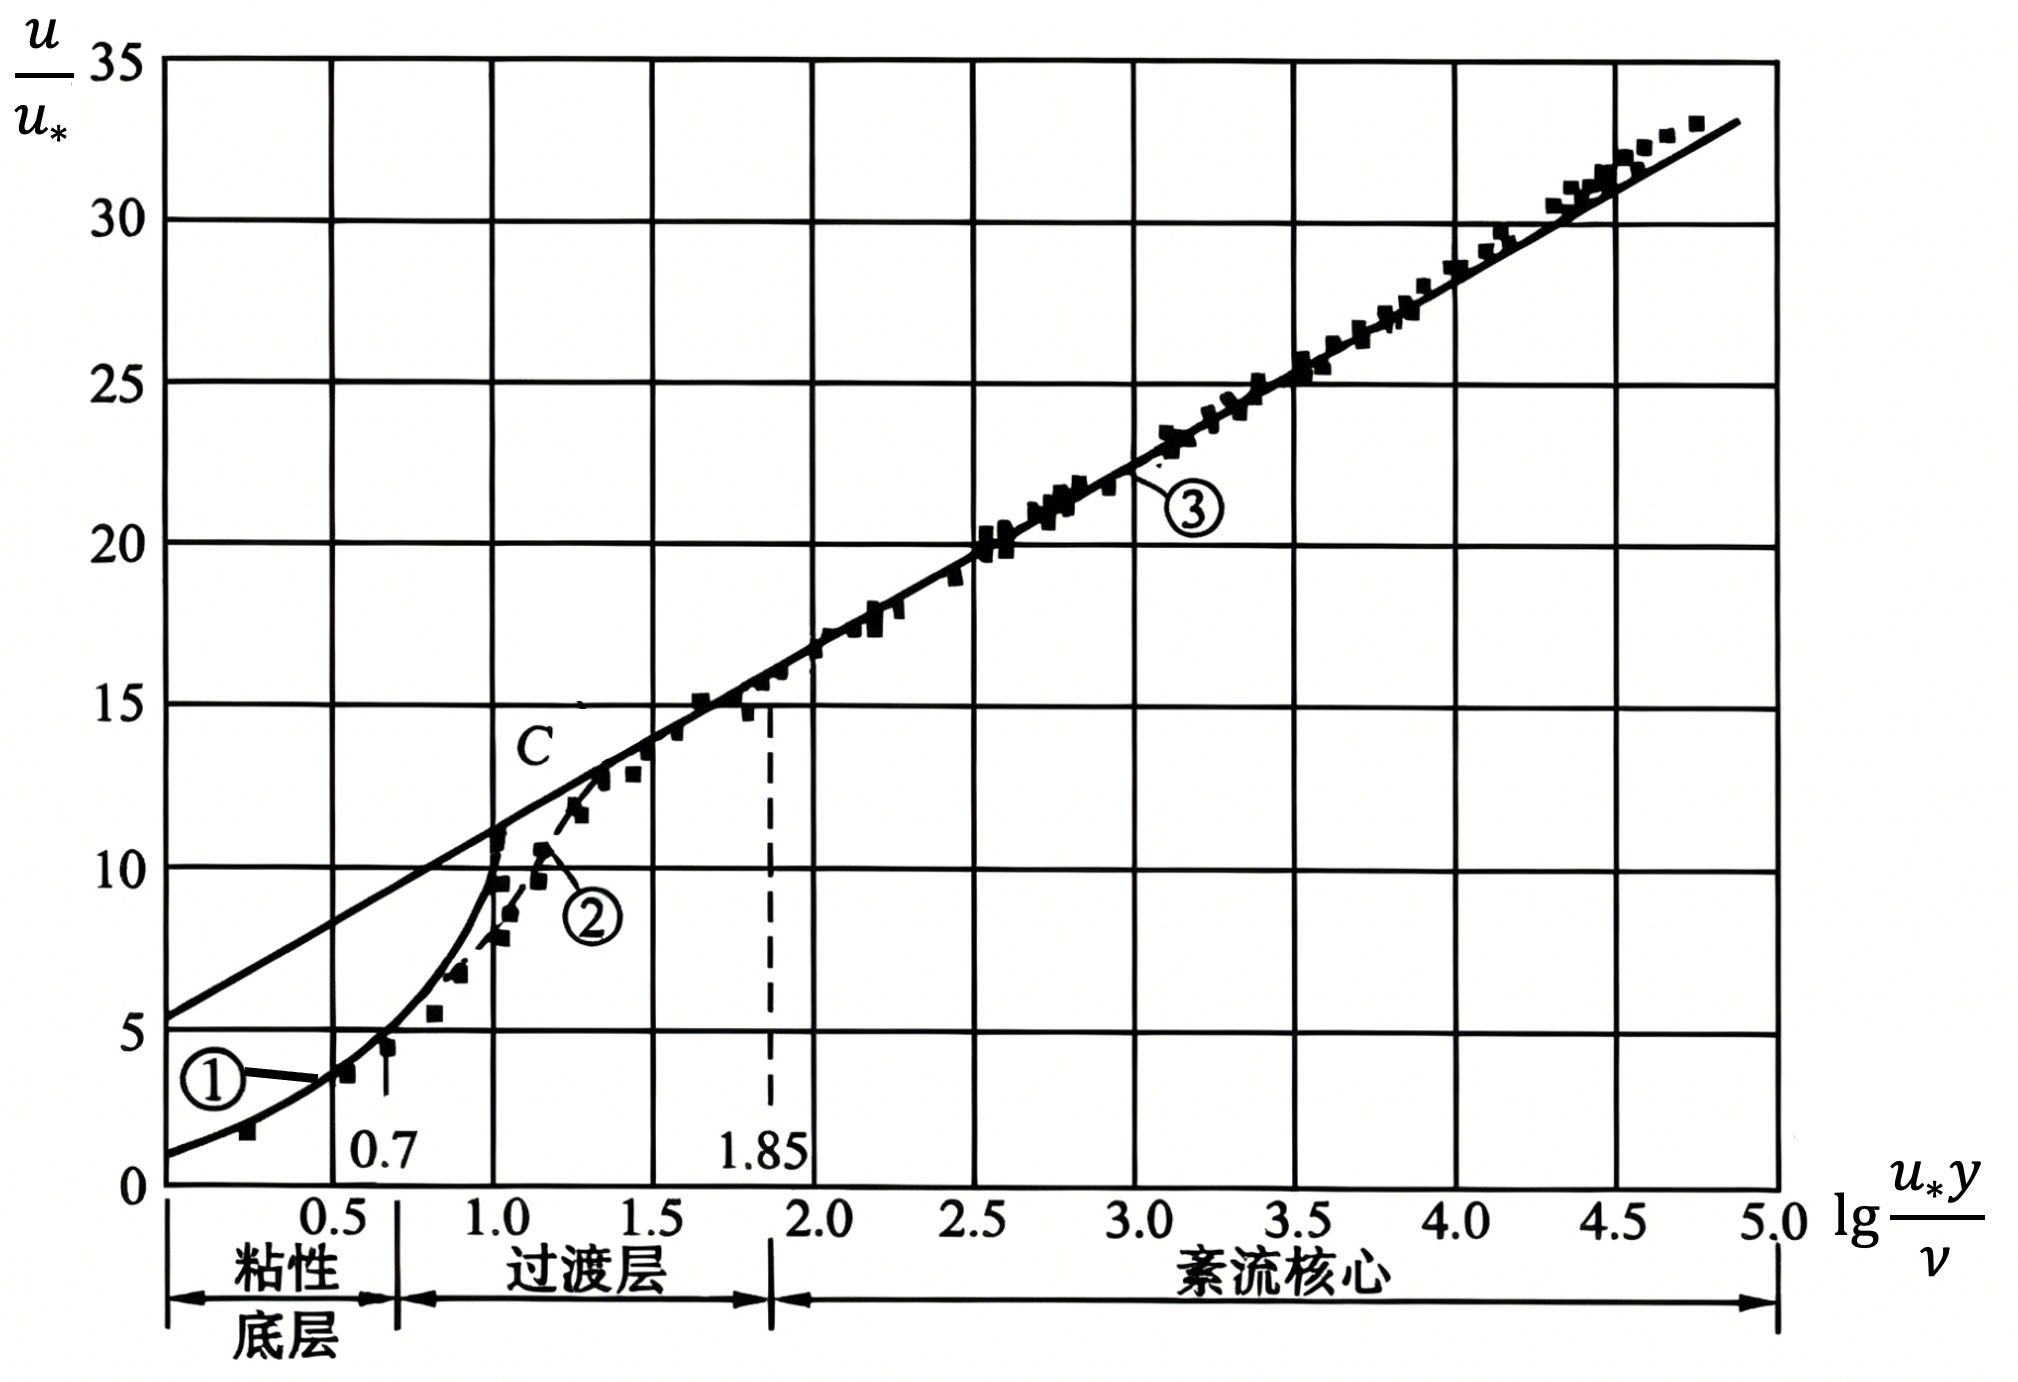
\includegraphics[width=0.72\textwidth,height=0.50\textheight,keepaspectratio]{slides_assets/fluid_deck05/loglaw-zones.png}\\
      {\scriptsize 图：源讲义原图}
  \end{center}
  \TLtakeaway{曲线交点 $y^+\approx11.6$ 落在过渡层内部；实际采用的粘性底层边界仍是 $y^+=5$。}
\end{frame}

\begin{frame}{D8a 壁面粗糙度：三区分类取决于 $u_*$}
  目的：同一根管子几何粗糙度固定，但水力上是否“光滑”取决于粗糙凸起相对近壁层是否被埋住。
  \begin{columns}[T]
    \column{0.57\textwidth}
      \[
        \begin{cases}
        \Delta\le\dfrac{5\nu}{u_*}, & \text{水力光滑管},\\[4pt]
        \dfrac{5\nu}{u_*}<\Delta\le\dfrac{70\nu}{u_*}, & \text{水力过渡粗糙},\\[6pt]
        \Delta>\dfrac{70\nu}{u_*}, & \text{水力粗糙管}.
        \end{cases}
        \tag{R33}
      \]
      $\Delta$ 是绝对粗糙度，$\Delta/d$ 是相对粗糙度。因为 $u_*$ 随 $\Rey$ 与阻力状态变化，同一管道低 $\Rey$ 时可能水力光滑，高 $\Rey$ 时可能水力粗糙。
    \column{0.43\textwidth}
      \centering
      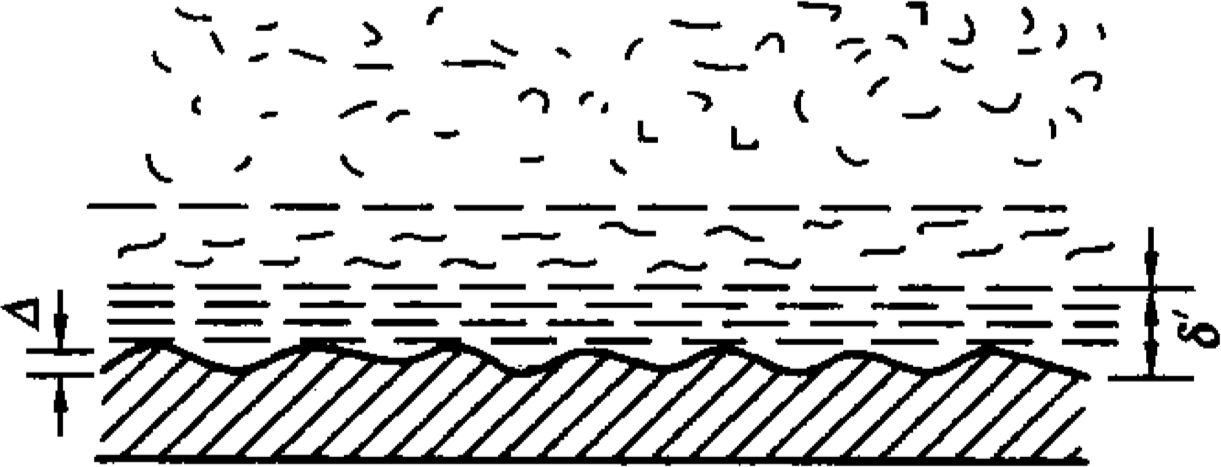
\includegraphics[width=\linewidth,height=\textheight,keepaspectratio]{slides_assets/fluid_deck05/roughness.png}\\
      {\scriptsize 图：源讲义原图}
  \end{columns}
  \TLtakeaway{“光滑/粗糙”在这里是水力分类，不只是肉眼摸起来光不光滑。}
\end{frame}

\begin{frame}{D8b 粗糙管对数律：用 $\Delta$ 作长度标尺}
  目的：水力粗糙时，壁面凸起已经控制近壁交换；对数律中的无量纲距离改由 $y/\Delta$ 给出。
  \begin{columns}[T]
    \column{0.54\textwidth}
      \textbf{半经验公式（粗糙管对数律）（拟合尼古拉兹粗糙管实验数据，适用水力粗糙区）。}
      \[
        u^+=5.75\,\lg\!\left(\frac{y}{\Delta}\right)+8.5 .
        \tag{R34}
      \]
      与光滑管相比，斜率 $5.75$ 保持不变；常数和对数里的长度标尺发生变化。
    \column{0.46\textwidth}
      \centering
      \begin{tikzpicture}[xscale=0.80,yscale=0.68,>={Stealth[length=5pt]}]
        \draw[->,TLprimaryDark,thick] (0,0)--(5.0,0) node[right] {$\Rey$};
        \draw[->,TLprimaryDark,thick] (0,0)--(0,3.8) node[above] {$\lambda$};
        \draw[TLaccent,thick] (0.55,3.2) .. controls (1.35,2.2) and (2.0,1.55) .. (2.65,1.25);
        \draw[TLprimary,thick] (1.25,2.85) .. controls (2.45,2.05) and (3.15,1.70) .. (4.35,1.65);
        \draw[TLprimaryDark,thick] (2.5,3.15) .. controls (3.2,2.55) and (4.0,2.35) .. (4.6,2.32);
        \node[font=\scriptsize,TLaccent] at (1.0,1.25) {光滑};
        \node[font=\scriptsize,TLprimary] at (3.1,1.35) {过渡粗糙};
        \node[font=\scriptsize,TLprimaryDark] at (3.7,2.65) {粗糙};
        \node[TLinkSoft,font=\scriptsize,align=center,text width=4.6cm] at (2.6,-0.55)
          {示意 Moody 图：粗糙度越突出，高 $\Rey$ 下阻力越不再只随 $\Rey$ 下降。};
      \end{tikzpicture}
  \end{columns}
  \TLtakeaway{粗糙管对数律仍是半经验公式；它告诉我们粗糙区的近壁长度标尺从 $\nu/u_*$ 换成了 $\Delta$。}
\end{frame}

\begin{frame}{D9a 指数形式：用一条幂函数拟合整段剖面}
  目的：对数律理论性较强但使用不便；工程上常用幂函数直接拟合速度剖面，便于积分得到平均量。
  \begin{columns}[T]
    \column{0.52\textwidth}
      \textbf{半经验公式（指数律）（拟合实验数据，适用紊流核心区及工程近似剖面）。}
      \[
        \frac{u}{u_{\max}}=\left(\frac{y}{r_0}\right)^n,
        \qquad 0<n<1 .
        \tag{R35}
      \]
      这里 $y$ 从壁面量起，$r_0$ 为管半径，$u_{\max}$ 是管轴线最大时均流速。$\Rey$ 越大，$n$ 越小，剖面越钝。
    \column{0.48\textwidth}
      \centering
      \begin{tikzpicture}[scale=0.78,>={Stealth[length=5pt]}]
        \draw[TLprimaryDark,thick] (0,-1.25)--(0,1.25);
        \draw[TLprimaryDark,thick] (0,-1.25)--(3.7,-1.25);
        \draw[TLprimaryDark,thick] (0,1.25)--(3.7,1.25);
        \draw[TLaccent,thick,smooth,domain=-1:1,samples=90]
          plot({3.15*(1-abs(\x)^6)}, {1.25*\x});
        \draw[TLprimary,thick,dashed,smooth,domain=-1:1,samples=90]
          plot({3.15*(1-abs(\x)^3)}, {1.25*\x});
        \node[TLaccent,font=\scriptsize] at (2.6,0.82) {较小 $n$：更钝};
        \node[TLprimary,font=\scriptsize] at (1.5,-0.75) {较大 $n$};
        \draw[->,TLprimaryDark] (0,0)--(0.9,0) node[above] {$u$};
      \end{tikzpicture}
  \end{columns}
  \TLtakeaway{指数律是拟合公式，不是由混合长严格推导；它的好处是形式简单，适合估算平均速度与修正系数。}
\end{frame}

\begin{frame}{D9b 指数律如何连到 $\bar v,\alpha,\beta$}
  进度：上一帧给出 $u/u_{\max}=(y/r_0)^n$；本帧用圆管面积分说明表格中的比值从哪里来。\proofskipnote
  令 $s=y/r_0$，则 $r=r_0-y=r_0(1-s)$，面积元满足 $\rd A=2\pi r_0^2(1-s)\rd s$，而 $A=\pi r_0^2$。
  \[
    \frac{\bar v}{u_{\max}}
    =2\int_0^1s^n(1-s)\rd s
    =2\left(\frac{1}{n+1}-\frac{1}{n+2}\right)
    =\frac{2}{(n+1)(n+2)} .
    \tag{R36}
  \]
  与 Deck 4 的定义一致，
  \[
    \beta=\frac{2\int_0^1s^{2n}(1-s)\rd s}{(\bar v/u_{\max})^2},
    \qquad
    \alpha=\frac{2\int_0^1s^{3n}(1-s)\rd s}{(\bar v/u_{\max})^3}.
    \tag{R37}
  \]
  \TLtakeaway{$\alpha,\beta$ 越接近 $1$，说明断面速度越接近均匀；这与紊流剖面更钝的图像一致。}
\end{frame}

\begin{frame}{D9c 指数律参数表：$\Rey$ 越大，剖面越钝}
  下表采用水力学教材中常见的圆管紊流指数律典型值；源讲义的表格 OCR 缺失，本表按 (R36)--(R37) 与常用指数取值整理。
  \begin{center}
  \vspace{4pt}
  \footnotesize
  \setlength{\tabcolsep}{4pt}
  \renewcommand{\arraystretch}{1.08}
  \begin{tabular}{@{}ccccc@{}}
    \toprule
    $\Rey$ 量级 & 指数 $n$ & $u_{\max}/\bar v$ & $\alpha$ & $\beta$ \\
    \midrule
    $4.0\times10^3$ & $1/6$  & $1.26$ & $1.08$ & $1.03$ \\
    $1.0\times10^5$ & $1/7$  & $1.22$ & $1.06$ & $1.02$ \\
    $1.0\times10^6$ & $1/8$  & $1.20$ & $1.05$ & $1.02$ \\
    $2.0\times10^6$ & $1/9$  & $1.17$ & $1.04$ & $1.01$ \\
    $>3.0\times10^6$ & $1/10$ & $1.16$ & $1.03$ & $1.01$ \\
    \bottomrule
  \end{tabular}
  \end{center}
  \TLtakeaway{这张表呼应 Deck 4：紊流 $\Rey$ 越大，剖面越平坦，平均速度写法越接近真实断面动能与动量通量。}
\end{frame}

\TLsection{常见误区}

\begin{frame}{常见误区（一）：把瞬时层流公式搬到时均紊流}
  初学者常把“形式相似”误认为“物理相同”：层流瞬时场、紊流瞬时场、紊流时均场不能混用。
  \TLwarnblock{三个需要立刻纠正的判断}{
    \begin{itemize}
      \item 错把 $\tau=\mu\,\rd u/\rd y$ 用于紊流时均场；正确做法是另计雷诺应力。
      \item 错把 $\Rey$ 当成精确开关；实际是下临界较稳，上临界随扰动大幅波动。
      \item 错把 $u_*$ 当成某处实际速度；它只是由 $\tau_w$ 构造出的剪切速度标尺。
    \end{itemize}
  }
  \[
    \tau_{\text{时均紊流}}
    =\mu\frac{\rd \bar u}{\rd y}
    +\tau^{Re},\qquad
    \tau^{Re}=-\rho\,\overline{u'v'} .
    \tag{R38}
  \]
  \TLtakeaway{先问“这是瞬时量还是时均量”，再决定能不能使用熟悉公式。}
\end{frame}

\begin{frame}{常见误区（二）：把两个“过渡”说成同一件事}
  “恒定”“均匀”“过渡区”都有物理限定对象；漏掉限定对象，判断就会反过来。
  \TLwarnblock{两个语境型误区}{
    \begin{itemize}
      \item 错把“恒定/均匀紊流”理解为瞬时场不变；正确对象是时均场。
      \item 错把近壁“过渡层”理解为层流到紊流的“过渡区”；前者是缓冲层，后者是转捩区。
    \end{itemize}
  }
  \[
    5<y^+<70\quad(\text{近壁缓冲层})
    \qquad\ne\qquad
    \Rey_c<\Rey<\Rey'_{cr}\quad(\text{流态转捩}) .
    \tag{R39}
  \]
  \TLtakeaway{同一个词出现在不同物理层级中时，必须回到定义判断。}
\end{frame}

\TLsection{练习}

\begin{frame}{练习1 $\star$：圆管与明渠的雷诺数判别}
  \TLinfoblock{题目}{
    已知 $\rho=1000\,\mathrm{kg/m^3}$、$\nu=1.0\times10^{-6}\,\mathrm{m^2/s}$、$d=0.05\,\mathrm m$、$V=0.08\,\mathrm{m/s}$。先判圆管流态；再改成宽 $B=0.5\,\mathrm m$、水深 $h=0.1\,\mathrm m$ 的明渠，用 $R=A/\chi$ 与临界 $\Rey_{\mathrm{cr}}\approx580$ 判别。
  }
  \begin{itemize}
    \item 提示 1：圆管直接用 $\Rey=Vd/\nu$，这里用管径作参考长度。
    \item 提示 2：矩形明渠湿周不是 $B+2h$ 之外再加自由液面；自由液面不属于湿周。
    \item 提示 3：明渠判据换成以水力半径 $R$ 为参考长度的雷诺数。
  \end{itemize}
  \[
    \begin{aligned}
    \Rey_{\text{管}}&=\frac{Vd}{\nu},\\
    R_{\text{渠}}&=\frac{Bh}{B+2h},&
    \Rey_{\text{渠}}&=\frac{VR_{\text{渠}}}{\nu}.
    \end{aligned}
    \tag{R40}
  \]
  \TLtakeaway{雷诺数判别必须先说清参考长度；圆管用 $d$，明渠常用水力半径 $R$。}
\end{frame}

\begin{frame}{练习2 $\star\star$：由壁面切应力求近壁层厚度}
  \TLinfoblock{题目}{
    已知 $\tau_w=0.36\,\mathrm{Pa}$、$\rho=1000\,\mathrm{kg/m^3}$、$\nu=1.0\times10^{-6}\,\mathrm{m^2/s}$。求 $u_*=\sqrt{\tau_w/\rho}$；再用 $y^+=5$ 求 $\delta'=5\nu/u_*$，并按题面约定用 $y^+=70$ 求 $\delta=70\nu/u_*$。
  }
  \begin{itemize}
    \item 提示 1：$1\,\mathrm{Pa}=1\,\mathrm{kg/(m\cdot s^2)}$，所以 $\tau_w/\rho$ 的量纲是 $\mathrm{m^2/s^2}$。
    \item 提示 2：先算 $u_*=\sqrt{0.36/1000}=0.018974\cdots\,\mathrm{m/s}$，后续按 $0.019\,\mathrm{m/s}$ 参与数值计算。
    \item 提示 3：$\delta'$ 和 $\delta_{70}$ 都与 $u_*$ 成反比；壁面摩擦越强，近壁层越薄。
  \end{itemize}
  \[
    \begin{aligned}
    u_*&=\sqrt{\frac{\tau_w}{\rho}},&
    \delta'&=\frac{5\nu}{u_*},&
    \delta&=\frac{70\nu}{u_*}.
    \end{aligned}
    \tag{R41}
  \]
  \TLtakeaway{$u_*$ 只是速度标尺；它的用途是把壁面切应力转成 $y^+$ 与近壁层厚度。}
\end{frame}

\begin{frame}{练习3 $\star\star$：用光滑管对数律求局部流速}
  \TLinfoblock{题目}{
    光滑管紊流核心区可用半经验公式 $u^+=2.5\ln y^+ + 5.5$。已知 $u_*=0.04\,\mathrm{m/s}$、$\nu=1.0\times10^{-6}\,\mathrm{m^2/s}$，求距壁面 $y=0.01\,\mathrm m$ 处的当地时均流速 $u$。
  }
  \begin{itemize}
    \item 提示 1：先算无量纲壁面距离 $y^+=yu_*/\nu$，判断量级是否进入对数律区。
    \item 提示 2：这里 $\ln$ 是自然对数；本题使用 $\ln(400)=5.991$。
    \item 提示 3：最后用 $u=u^+u_*$ 把无量纲速度还原成有量纲速度。
  \end{itemize}
  \[
    y^+=\frac{yu_*}{\nu},\qquad
    u^+=2.5\ln y^+ +5.5,\qquad
    u=u^+u_*.
    \tag{R42}
  \]
  \TLtakeaway{对数律先给 $u^+$，不是直接给 $u$；最后必须乘回摩阻流速。}
\end{frame}

\begin{frame}{练习4 $\star\star\star$：由粗糙度判别壁面公式}
  \footnotesize
  \TLinfoblock{题目}{
    圆管紊流中，$d=0.1\,\mathrm m$、$k_s=0.046\,\mathrm{mm}$、$\nu=1.0\times10^{-6}\,\mathrm{m^2/s}$、$u_*=0.05\,\mathrm{m/s}$。用 $k_s^+=k_su_*/\nu$ 判断水力分区，并写出应选的壁面速度公式。
  }
  \begin{itemize}
    \item 提示 1：先统一单位，$0.046\,\mathrm{mm}=0.046\times10^{-3}\,\mathrm m$。
    \item 提示 2：判据为 $k_s^+<5$ 光滑，$5\le k_s^+\le70$ 过渡，$k_s^+>70$ 粗糙。
    \item 提示 3：光滑管选 $u^+=2.5\ln y^+ +5.5$；粗糙管才改用粗糙律。
  \end{itemize}
  \[
    k_s^+=\frac{k_su_*}{\nu},\qquad
    \begin{cases}
    k_s^+<5, & \text{水力光滑},\\
    k_s^+>70, & \text{水力粗糙}.
    \end{cases}
    \tag{R43}
  \]
  \TLtakeaway{几何粗糙不等于水力粗糙；关键是 $k_s$ 相对 $\nu/u_*$ 是否足够大。}
\end{frame}

\TLsection{延伸与文献注记}

\begin{frame}{本讲义出处与历史人物}
  本 deck 对应源讲义第五章 5.1--5.2；这些经验公式背后是一条从实验观察到半经验封闭的历史线索。
  \begin{center}
  \vspace{4pt}
  \footnotesize
  \setlength{\tabcolsep}{3pt}
  \renewcommand{\arraystretch}{1.06}
  \begin{tabular}{@{}p{0.16\textwidth}p{0.28\textwidth}p{0.46\textwidth}@{}}
    \toprule
    人物 & 年代与关键词 & 本讲义中的位置 \\
    \midrule
    Reynolds & 1883，雷诺实验 & 确立 $\Rey$ 与层流/紊流判别语言 \\
    Boussinesq & 1877，涡粘假设 & 把雷诺应力写成类似粘性应力的形式 \\
    Prandtl & 1925，混合长理论 & 用 $l_m$ 封闭雷诺切应力 \\
    Kármán & 对数律常数 $\kappa\approx0.41$ & 给近壁对数律的通用斜率 \\
    Nikuradse & 1933，粗糙管实验 & 支撑光滑、过渡、粗糙分区 \\
    \bottomrule
  \end{tabular}
  \end{center}
  \TLtakeaway{本章公式多为半经验公式；它们的可靠性来自“物理假设 + 实验拟合”的组合。}
\end{frame}

\begin{frame}{RANS 与湍流模型：为什么还要建模}
  雷诺平均把瞬时速度拆成时均值和脉动值，但平均之后会产生新的未知量；这就是湍流模型的入口。
  \[
    \text{RANS 方程}
    \quad+\quad
    \tau_{ij}^{Re}=-\rho\,\overline{u_i'u_j'}
    \quad\Longrightarrow\quad
    \text{方程组不封闭}.
    \tag{R44}
  \]
  \begin{center}
  \vspace{2pt}
  \footnotesize
  \setlength{\tabcolsep}{4pt}
  \begin{tabular}{@{}p{0.25\textwidth}p{0.25\textwidth}p{0.38\textwidth}@{}}
    \toprule
    模型语言 & 思想 & 工程备注 \\
    \midrule
    Boussinesq 涡粘模型 & 用 $\eta$ 近似雷诺应力 & 把复杂交换写成“有效粘度” \\
    混合长模型 & $l_m=\kappa y$ 型代数封闭 & 简单，但依赖壁面经验 \\
    $k$--$\varepsilon$ 模型 & 两个输运方程 & 工程 CFD 中使用非常广泛 \\
    壁函数 & 不解析最薄近壁层 & 常配 $y^+=30$--$100$ 网格 \\
    \bottomrule
  \end{tabular}
  \end{center}
  精解析壁面通常要求第一层网格 $y^+\approx1$；壁函数法则把近壁细节交给经验公式。
  \TLtakeaway{RANS 的核心困难不是平均本身，而是平均后出现的雷诺应力需要封闭。}
\end{frame}

\begin{frame}{推荐教材与延伸阅读}
  外部资料只用于深化；本 deck 已经把 5.1--5.2 所需的基本定义、推导和算例写在页内。
  \begin{center}
  \vspace{4pt}
  \footnotesize
  \setlength{\tabcolsep}{3pt}
  \renewcommand{\arraystretch}{1.05}
  \begin{tabular}{@{}p{0.28\textwidth}p{0.24\textwidth}p{0.39\textwidth}@{}}
    \toprule
    资料 & 适合用途 & 阅读建议 \\
    \midrule
    闻德荪《工程流体力学》 & 本课程基础 & 先用它对齐中文水力学术语 \\
    Pope, \emph{Turbulent Flows} & 深入湍流理论 & 适合学完 N-S 与统计平均后再读 \\
    White, \emph{Fluid Mechanics} & 工程应用 & 对管流、摩阻和量纲分析很友好 \\
    维基百科与视频课程 & 可视化补充 & 可选深化，不作为必读资料 \\
    \bottomrule
  \end{tabular}
  \end{center}
  \[
    \text{本讲义主线}
    \longrightarrow
    \text{教材例题}
    \longrightarrow
    \text{湍流专著}.
    \tag{R45}
  \]
  \TLtakeaway{先把 $\Rey$、雷诺应力、$u_*$、$y^+$ 和对数律读通，再进入更完整的湍流理论。}
\end{frame}

\TLsection{术语速查}

\begin{frame}{术语速查（一）：流态、平均与雷诺应力}
  \begin{center}
  \vspace{4pt}
  \footnotesize
  \setlength{\tabcolsep}{1.8pt}
  \renewcommand{\arraystretch}{1.04}
  \begin{tabular}{@{}lll@{}}
    \toprule
    中文术语 & English term & 简要说明 \\
    \midrule
    层流 & laminar flow & 分层滑动，横向掺混弱 \\
    紊流（湍流） & turbulent flow & 无序脉动，横向掺混强 \\
    雷诺数 & Reynolds number & $\Rey=Vd/\nu$ \\
    上/下临界雷诺数 & \shortstack[l]{upper/lower\\critical Re} & 上临界受扰动影响大 \\
    时均流速 & \shortstack[l]{time-averaged\\velocity} & $\bar u=\lim_T T^{-1}\int u\,\rd t$ \\
    脉动流速 & \shortstack[l]{fluctuation\\velocity} & $u'=u-\bar u$ \\
    雷诺应力 & Reynolds stress & $\tau^{Re}=-\rho\overline{u'v'}$ \\
    涡粘系数 & eddy viscosity & $\eta$，Boussinesq 假设 \\
    混合长 & mixing length & $l_m=\kappa y$ 近壁模型 \\
    \bottomrule
  \end{tabular}
  \end{center}
  \TLtakeaway{第一组术语回答“紊流怎样描述、为什么时均后还会多出应力”。}
\end{frame}

\begin{frame}{术语速查（二）：近壁尺度、壁面律与粗糙度}
  \begin{center}
  \vspace{4pt}
  \footnotesize
  \setlength{\tabcolsep}{1.8pt}
  \renewcommand{\arraystretch}{1.04}
  \begin{tabular}{@{}lll@{}}
    \toprule
    中文术语 & English term & 简要说明 \\
    \midrule
    摩阻流速 & friction velocity & $u_*=\sqrt{\tau_w/\rho}$ \\
    粘性底层 & viscous sublayer & $y^+<5$ \\
    过渡层（缓冲层） & buffer layer & $5<y^+<70$ \\
    对数律 & log law & $u^+=2.5\ln y^++5.5$ \\
    壁面律 & law of the wall & 近壁无量纲速度剖面 \\
    水力光滑 & \shortstack[l]{hydraulically\\smooth} & $k_s^+<5$ \\
    水力粗糙 & \shortstack[l]{hydraulically\\rough} & $k_s^+>70$ \\
    相对粗糙度 & \shortstack[l]{relative\\roughness} & $k_s/d$ \\
    \bottomrule
  \end{tabular}
  \end{center}
  \TLtakeaway{第二组术语回答“距壁距离怎样无量纲化、何时选光滑律或粗糙律”。}
\end{frame}

\appendix

\begin{frame}{附录：练习1 解答}
  \label{A1}
  \footnotesize
  圆管用管径 $d$ 作参考长度：
  \[
    \Rey_{\text{管}}
    =\frac{Vd}{\nu}
    =\frac{0.08\times0.05}{1.0\times10^{-6}}
    =4000 .
    \tag{R46}
  \]
  因为 $4000>2300$，按圆管工程判据可判为紊流。明渠先求过水面积、湿周和水力半径：
  \[
    A=Bh=0.5\times0.1=0.05\,\mathrm{m^2},\quad
    \chi=B+2h=0.5+0.2=0.7\,\mathrm m,\quad
    R=\frac{A}{\chi}=\frac{0.05}{0.7}=0.0714\,\mathrm m .
    \tag{R47}
  \]
  \[
    \Rey_{\text{渠}}
    =\frac{VR}{\nu}
    =\frac{0.08\times0.0714}{1.0\times10^{-6}}
    \approx5714 .
    \tag{R48}
  \]
  \TLresultblock{答案}{
    \[
      \boxed{\Rey_{\text{管}}=4000\ \text{紊流},\qquad
      R=0.0714\,\mathrm m,\qquad
      \Rey_{\text{渠}}\approx5714\ \text{紊流}.}
    \]
  }
\end{frame}

\begin{frame}{附录：练习2 解答}
  \label{A2}
  \footnotesize
  先把壁面切应力换成速度标尺：
  \[
    u_*=\sqrt{\frac{\tau_w}{\rho}}
    =\sqrt{\frac{0.36}{1000}}
    =0.018974\cdots\,\mathrm{m/s}
    \approx0.019\,\mathrm{m/s}.
    \tag{R49}
  \]
  后续按题面指定的 $u_*=0.019\,\mathrm{m/s}$ 参与数值计算。粘性底层厚度为
  \[
    \delta'=\frac{5\nu}{u_*}
    =\frac{5\times10^{-6}}{0.019}
    =2.63\times10^{-4}\,\mathrm m .
    \tag{R50}
  \]
  按本题约定，用 $y^+=70$ 定义的厚度为
  \[
    \delta=\frac{70\nu}{u_*}
    =\frac{70\times10^{-6}}{0.019}
    =3.68\times10^{-3}\,\mathrm m .
    \tag{R51}
  \]
  \TLresultblock{答案}{
    \[
      \boxed{u_*=0.019\,\mathrm{m/s},\quad
      \delta'=2.63\times10^{-4}\,\mathrm m,\quad
      \delta=3.68\times10^{-3}\,\mathrm m.}
    \]
  }
\end{frame}

\begin{frame}{附录：练习3 解答}
  \label{A3}
  \footnotesize
  先计算无量纲壁面距离：
  \[
    y^+=\frac{yu_*}{\nu}
    =\frac{0.01\times0.04}{1.0\times10^{-6}}
    =400 .
    \tag{R52}
  \]
  用自然对数形式的光滑管对数律：
  \[
    u^+=2.5\ln(400)+5.5
    =2.5\times5.991+5.5
    =14.977+5.5
    =20.48 .
    \tag{R53}
  \]
  乘回摩阻流速得到当地时均流速：
  \[
    u=u^+u_*
    =20.48\times0.04
    =0.819\,\mathrm{m/s}.
    \tag{R54}
  \]
  \TLresultblock{答案}{
    \[
      \boxed{y^+=400,\qquad u^+=20.48,\qquad u\approx0.819\,\mathrm{m/s}.}
    \]
  }
\end{frame}

\begin{frame}{附录：练习4 解答}
  \label{A4}
  \footnotesize
  先把粗糙度统一成米：
  \[
    k_s=0.046\,\mathrm{mm}=0.046\times10^{-3}\,\mathrm m .
    \tag{R55}
  \]
  计算粗糙度的壁面单位：
  \[
    k_s^+=\frac{k_su_*}{\nu}
    =\frac{0.046\times10^{-3}\times0.05}{1.0\times10^{-6}}
    =2.3 .
    \tag{R56}
  \]
  因为 $2.3<5$，该工况属于水力光滑区，应使用光滑管对数律：
  \[
    u^+=2.5\ln y^+ +5.5 .
    \tag{R57}
  \]
  \TLresultblock{答案}{
    \[
      \boxed{k_s^+=2.3<5,\quad \text{水力光滑，适用 }u^+=2.5\ln y^+ +5.5.}
    \]
  }
\end{frame}

\end{document}
